\documentclass[letterpaper,twocolumn,10pt]{article}
\usepackage{usenix2019_v3}

% conference specific style
% \usepackage[11pt,nocopyright]{sigmin}
% \usepackage[square,comma,numbers,sort&compress]{natbib}
\usepackage{tikz}
\usepackage{booktabs}
\usepackage[square,comma,numbers,sort&compress]{natbib}

\usepackage{amsmath}
\usepackage{algorithm}
% \usepackage[cache=true,outputdir=./latex.out]{minted}
\usepackage{hyperref}
\usepackage{algpseudocode}
\usepackage{pgfplots}  % 支持 pgfplots 插图
\pgfplotsset{compat=1.17}  % 设置 pgfplots 版本
\usepgfplotslibrary{groupplots}

% inlined bib file
\usepackage{filecontents}

\usepackage{color, xcolor}
\usepackage[colorinlistoftodos,prependcaption,textsize=tiny]{todonotes}


%-------------------------------------------------------------------------------
\begin{filecontents}{\jobname.bib}
    %-------------------------------------------------------------------------------
    @Book{arpachiDusseau18:osbook,
      author =       {Arpaci-Dusseau, Remzi H. and Arpaci-Dusseau Andrea C.},
      title =        {Operating Systems: Three Easy Pieces},
      publisher =    {Arpaci-Dusseau Books, LLC},
      year =         2015,
      edition =      {1.00},
      note =         {\url{http://pages.cs.wisc.edu/~remzi/OSTEP/}}
    }
    @InProceedings{waldspurger02,
      author =       {Waldspurger, Carl A.},
      title =        {Memory resource management in {VMware ESX} server},
      booktitle =    {USENIX Symposium on Operating System Design and
                      Implementation (OSDI)},
      year =         2002,
      pages =        {181--194},
      note =         {\url{https://www.usenix.org/legacy/event/osdi02/tech/waldspurger/waldspurger.pdf}}}
    \end{filecontents}

% common packages
\usepackage[english]{babel}
\usepackage{blindtext}
% \usepackage{algorithm}
% \usepackage{algpseudocode}
\usepackage{graphicx}
% to be able to draw some self-contained figs
\usepackage{tikz}
\usepackage{amsmath}
\usepackage{enumitem}

% inlined bib file
\usepackage{filecontents}

\usepackage{MnSymbol}
\usepackage[english]{babel}
\usepackage{blindtext}
\usepackage{color}
\usepackage{xspace}
\usepackage{xcolor}
% \usepackage[linesnumbered,ruled,vlined]{algorithm2e}
\usepackage{caption}
\usepackage{multirow}
\usepackage{gensymb}
\usepackage{flushend}
\usepackage{newtxmath}
\usepackage{url}
\usepackage[normalem]{ulem}


\newcommand{\sys}{\mbox{\textsc{Select-N}}\xspace}
\newcommand{\syss}{\mbox{\textsc{Select-N's}}\xspace}

\newcommand{\deepspeed}{DeepSpeed\xspace}
\newcommand{\flexgen}{FlexGen\xspace}

\newcommand{\Interval}{Offloading interval\xspace}
\newcommand{\interval}{offloading interval\xspace}
\newcommand{\intervals}{offloading intervals\xspace}

\newcommand{\oflayer}{offloaded layer\xspace}

\newcommand{\analyzer}{analyzer\xspace}
\newcommand{\Record}{Record\xspace}
\newcommand{\record}{record\xspace}
\newcommand{\records}{records\xspace}



% Figure command
\newcommand{\insertFigure}[2]{
    \begin{figure}[t!]
%\setlength{\abovecaptionskip}{0pt}
%\setlength{\belowcaptionskip}{0pt}
        \centering
        \includegraphics[width=\linewidth]{figures/#1.pdf}
	\vspace{-6mm}
        \caption{\small #2}
	\vspace{-3mm}
        \label{fig:#1}
    \end{figure}
}

\newcommand{\insertWideFigure}[2]{

    \begin{figure*}[ht!]
%\setlength{\abovecaptionskip}{0pt}
%\setlength{\belowcaptionskip}{0pt}
        \centering
        \includegraphics[width=\textwidth]{figures/#1.pdf}
	\vspace{-6mm}
        \caption{\small #2}
	\vspace{-3mm}
        \label{fig:#1}
    \end{figure*}

}

\newcommand*\circledsmall[1]{\tikz[baseline=(char.base)]{
            \node[shape=circle,fill=darkgray,inner sep=0.5pt] (char) {\small\textcolor{white}{#1}};}}

\newcommand*\circled[1]{\tikz[baseline=(char.base)]{
            \node[shape=circle,fill=darkgray,inner sep=0.5pt] (char) {\textcolor{white}{#1}};}}

%%%% for tighter bullets
\newcommand{\squishlist}{
 \begin{list}{$\bullet$}
  { \setlength{\itemsep}{0pt}
     \setlength{\parsep}{0pt}
     \setlength{\topsep}{3pt}
     \setlength{\partopsep}{0pt}
     \setlength{\leftmargin}{1.5em}
     \setlength{\labelwidth}{1em}
     \setlength{\labelsep}{0.5em} } }
     
%%%% for tighter numbers
\newcommand{\squishnums}{
 \begin{list}{$\bullets$}
  { \setlength{\itemsep}{0pt}
     \setlength{\parsep}{3pt}
     \setlength{\topsep}{3pt}
     \setlength{\partopsep}{0pt}
     \setlength{\leftmargin}{1.5em}
     \setlength{\labelwidth}{1em}
     \setlength{\labelsep}{0.5em} } }

\newcommand{\squishlisttwo}{
 \begin{list}{$\bullet$}
  { \setlength{\itemsep}{0pt}
     \setlength{\parsep}{0pt}
    \setlength{\topsep}{0pt}
    \setlength{\partopsep}{0pt}
    \setlength{\leftmargin}{2em}
    \setlength{\labelwidth}{1.5em}
    \setlength{\labelsep}{0.5em} } }

\newcommand{\squishend}{
  \end{list}  }


\newcommand{\betterparagraph}[1]{\textbf{#1.}}


% Sections
\def\sectionautorefname{Sec.}

\renewcommand*\sectionautorefname{\Snospace}
\def\subsectionautorefname{Sec.}
\def\subsubsectionautorefname{Sec.}

% Figures
\def\figureautorefname{Fig.}


\newcommand{\greencheck}{{\color{ForestGreen}\checkmark}}
\newcommand{\orangecheck}{{\color{orange}\checkmark}}
\newcommand{\redcheck}{{\color{red}\xmark}}

\newcommand{\NMName}[0]{\textsc{Einsum}~}
\newcommand{\NMNameTitle}[0]{Einsum}

\newcommand{\NMNamenospace}[0]{\textsc{Einsum}}

\newcommand{\NMNameOff}[0]{\textsc{Einsum} (near DRAM)~}
\newcommand{\NMNameOffTitle}[0]{\textsc{Einsum} (near DRAM)}

\newcommand{\NMNameOffnospace}[0]{\textsc{Einsum} (near DRAM)}

\newcommand{\TitleName}[0]{\textsc{Harp}~}

\newcommand{\TitleNamenospace}[0]{\textsc{Harp}}

\newcommand{\HHPName}[0]{\textsc{Harp}~}

\newcommand{\HHPNamenospace}[0]{\textsc{Harp}}

\newcommand{\NoCName}[0]{\textsc{In-switch}~}

\newcommand{\NoCNamenospace}[0]{\textsc{In-switch}}

\newcommand{\TODO}[1]{\textcolor{red}{TODO::: #1}}
\newcommand{\RG}[1]{{\color{orange}\bfseries [RG::: #1]}}
\newcommand{\TK}[1]{{\color{teal}\bfseries [Tushar::: #1]}} 
\newcommand{\MP}[1]{{\color{olive}\bfseries [Michael::: #1]}}

\newcommand{\fixme}[1]{{{\color{blue} #1}}}


\newcommand{\cmark}{\ding{51}}%
\newcommand{\xmark}{\ding{55}}%

%\renewcommand{\hl}{}

%\begin{comment}
\renewcommand{\RG}[1]{\ignorespaces}

\renewcommand{\TK}[1]{\ignorespaces}

\renewcommand{\TODO}[1]{\ignorespaces}

%\end{comment}


\newcommand{\insertFigurePartnn}[2]{
    \begin{figure}[t]
%\setlength{\abovecaptionskip}{0pt}
%\setlength{\belowcaptionskip}{0pt}
        \centering
        \includegraphics[width=0.85\linewidth]{figures/#1.pdf}
	\vspace{-2mm}
        \caption{#2}
	\vspace{0mm}
        \label{fig:#1}
    \end{figure}
}

% Sections
\renewcommand*\sectionautorefname{\Snospace}
\def\sectionautorefname{Sec.}
\def\subsectionautorefname{Sec.}
\def\subsubsectionautorefname{Sec.}

% Figures
\def\figureautorefname{Fig.}

\def\algorithmautorefname{Alg.}

\def\tableautorefname{Table}


\newcommand{\insertWideFigureScaled}[3]{

    \begin{figure*}[ht!]
%\setlength{\abovecaptionskip}{0pt}
%\setlength{\belowcaptionskip}{0pt}
        \centering
        \includegraphics[width=#3\textwidth]{figures/#1.pdf}
	\vspace{-3mm}
        \caption{\small #2}
	\vspace{0mm}
        \label{fig:#1}
    \end{figure*}

}

\newcommand{\insertFigureScaled}[3]{

    \begin{figure}[t!]
%\setlength{\abovecaptionskip}{0pt}
%\setlength{\belowcaptionskip}{0pt}
        \centering
        \includegraphics[width=#3\linewidth]{figures/#1.pdf}
	\vspace{-3mm}
        \caption{\small #2}
	\vspace{0mm}
        \label{fig:#1}
    \end{figure}

}
% \gdef\therev{24e5157}
\gdef\thedate{2025-01-15 01:32:46 +0800}


\begin{document}

%don't want date printed
\date{}

% make title bold and 14 pt font (Latex default is non-bold, 16 pt)
% \title{Latency-SLO-Aware Memory Offloading for Large Language Model Inference}

% arXiv title
\title{Memory Offloading for Large Language Model Inference with Latency SLO Guarantees}

%for single author (just remove % characters)
\author{
{\rm Chenxiang Ma}\\
Peking University
\and
{\rm Zhisheng Ye}\\
Peking University
\and
{\rm Hanyu Zhao}\\
Alibaba Cloud Computing
\and
{\rm Zehua Yang}\\
Peking University
\and
{\rm Tianhao Fu}\\
Peking University
\and
{\rm Jiaxun Han}\\
Peking University
\and
{\rm Jie Zhang}\\
Peking University
\and
{\rm Yingwei Luo}\\
Peking University
\and
{\rm Xiaolin Wang}\\
Peking University
\and
{\rm Zhenlin Wang}\\
Michigan Tech
\and
{\rm Yong Li}\\
Alibaba Cloud Computing
\and
{\rm Diyu Zhou}\\
Peking University
} % end author

\maketitle

\sloppy

Vision-Language Models (VLMs) occasionally generate outputs that contradict input images, constraining their reliability in real-world applications. While visual prompting is reported to suppress hallucinations by augmenting prompts with relevant area inside an image, the effectiveness in terms of the area remains uncertain. This study analyzes success and failure cases of Attention-driven visual prompting in object hallucination, revealing that preserving background context is crucial for mitigating object hallucination.

Gaussian Processes (GPs) \citep{kolmogorov1940wienersche,rasmussen2006gaussian} are an important class of stochastic processes used in machine learning and statistics, with use cases including spatial data analysis \citep{liu2021missing}, time series forecasting \citep{girard2002gaussian}, bioinformatics \citep{luo2023diseasegps} and Bayesian optimization \citep{frazier2018tutorial}. GPs offer a non-parametric framework for modeling distributions over functions, enabling both flexibility and uncertainty quantification. These capabilities, combined with the ability to incorporate prior knowledge and specify relationships by choice of kernel function, make Gaussian Processes effective for both regression and classification.

However, GPs have substantial computational and memory bottlenecks. Both training and inference require computing the action of the inverse kernel Gram matrix, while training requires computing its log-determinant: both are $O(n^3)$ operations with sample size $n$. Further, storing the full Gram matrix requires $O(n^2)$ memory. These bottlenecks require scalable approximations for larger datasets.

Structured Kernel Interpolation (SKI) \cite{wilson2015kernel} helps scale Gaussian Processes (GPs) to large datasets by approximating the kernel matrix using interpolation on a set of inducing points. For stationary kernels, this requires $O(n+m \log m)$ computational complexity. The core idea is to express the original kernel as a combination of interpolation functions and a kernel matrix defined on a set of inducing points. However, despite its effectiveness, popularity (over $600$ citations, a large number for a GP paper) and high quality software availability (\cite{gardner2018gpytorch} has 3.5k stars on github), it currently lacks theoretical analysis. A key initial question is, given a fixed error bound for the SKI Gram matrix and use of cubic convolutional interpolation, how many inducing points are required to achieve that error bound? Given the required value of $m$ as a function of $n$, for what error tolerance is $O(n+m\log m)$ still linear? Following this, what do these errors imply for hyperparameter estimation and posterior inference?

\begin{table*}[h]
\centering
\begin{tabular}{|l|l|}
\hline
\textbf{Quantity} & \textbf{Bound} \\
\hline
SKI kernel error & $O(\frac{c^{2d}}{m^{3/d}})$ \\
\hline
SKI Gram matrix error & $O(\frac{nc^{2d}}{m^{3/d}})$ \\
\hline
SKI cross-kernel matrix error & $O(\frac{\max(n,T)c^{2d}}{m^{3/d}})$ \\
\hline
SKI score function error & $O(\frac{\sqrt{p}n^{2}c^{4d}}{m^{3/d}})$ \\
\hline
SKI posterior mean error & $O(c^{2d}\frac{\max(T,n)+\sqrt{Tn}n}{m^{3/d}})$ \\
\hline
SKI posterior covariance error & $O(\frac{Tn^{2}mc^{4d}+\sqrt{Tn}mc^{4d}\max(T,n)}{m^{3/d}})$ \\
\hline
\end{tabular}
\caption{Summary of Theoretical Results when using SKI with convolutional cubic interpolation. This shows the rate at which the error of using SKI (vs the exact kernel) grows as a function of important variables. Here $n$ and $T$ are the train/test sample sizes, $d$ is the dimensionality, $m$ the number of inducing points, $p$ is the number of hyperparameters and $c>0$ is a constant. Most importantly, the Gram matrix error grows linearly with the sample size, exponentially with the dimension while decaying at an $m^{3/d}$ rate in the inducing points.}
\label{table:theoretical_results}
\end{table*}

In this paper, we begin to bridge the gap between practice and a theoretical understanding of SKI. We have three primary contributions: 1) The first error analysis for the SKI kernel and relevant quantities, including the SKI gram matrix's spectral norm error. Based on this we provide \textit{a practical guide to select the number of inducing points}: they should grow as $n^{d/3}$ to control error. 2) SKI hyperparameter estimation analysis. 3) SKI inference analysis: the error of the GP posterior means and variances at test points. We find two interesting results: 1) we identify two dimensionality regimes relating SKI Gram matrix error to computational complexity. For $d\leq 3$, for \textit{any} fixed spectral norm error, we can achieve it in linear time using SKI with a sufficient sample size. For $d>3$, the error must \textit{increase} with the sample size to maintain our guarantee of linear time. 2) For a $\mu$-smooth log-likelihood, gradient ascent on the SKI log-likelihood will approach a neighborhood of a stationary point of the true log-likelihood at a $O\left(\frac{1}{K}\right)$ rate, with the neighborhood size determined by the SKI score function's error, which aside from the response variables grows \textit{linearly} with the sample size when increasing inducing points as we suggested. To obtain this, we leverage a recent result \cite{stonyakin2023stopping} from the inexact gradient descent \cite{daspremont2008smooth,devolder2014first} literature.

% By our downstream analysis, this implies that for small dimensionality and kernels exhibiting desirable regularity conditions, we can have arbitrarily small error in the SKI Gram matrix, in our estimated parameters and in posterior inference all in linear time as long as the sample size is sufficiently large.

In section \ref{sec:related} we describe related work. In section \ref{sec:ski-background} we give a brief background on SKI. In section \ref{sec:important-quantities} we bound the error of important quantities: specifically the SKI kernel, Gram matrix and cross-kernel matrix errors. In section \ref{sec:gp-applications} we use these to analyze the error of the SKI MLE and posteriors. We conclude in section \ref{sec:discussion} by summarizing our results and discussing limitations and future work.
\section{Background and Related Work}
\label{sec:background}
% \subsection{Text Data Summarization}
% % Text summarization is a basic task in NLP domains that aims to compress original articles into a few sentences while retaining essential information and meaning. Overall, text summarization can be divided into extractive summarization and abstractive summarization.


% Text data summarization significantly enhances the efficiency of data processing, storing, and retrieving by extracting and generating concise summaries. For example, it helps search engines better determine the relevance between queries and results~\cite{MarketBrew2024SEO}. Overall, text summarization can be divided into extractive summarization and abstractive summarization.

% % Over the past few years, various approaches have been developed to enhance the performance of news summarization~\cite{zhou-etal-2018-neural-document,dong-etal-2018-banditsum,zhang-etal-2018-neural,t5,pegasus,brio,lewis-etal-2020-bart}. 

% % \subsubsection{Extractive Summarization}
% Extractive summarization is selecting the most relevant sentences from the original text to form a summary. This can ensure the relevance and faithfulness of the summary but may result in a lack of coherence or some redundant information. Early methods often use statistical or graph-based approaches to measure sentence importance. Luhn~\cite{luhn1958automatic} proposed a method based on word frequency statistics to select the most important sentences from a text. And TextRank~\cite{mihalcea2004textrank} is a graph-based ranking algorithm that represents the text as a graph, where nodes represent basic units of the text (such as words or sentences), and edges represent relationships between these units. Through the structure of the graph and the strength of connections between nodes, the TextRank algorithm can evaluate the importance of each node. BanditSum~\cite{dong-etal-2018-banditsum} addressed sentence selection by framing it as a contextual bandit problem. With the development of word embeddings~\cite{mikolov2013word2vec}, many works have started using semantic information to select sentences. For instance, NEUSUM~\cite{zhou-etal-2018-neural-document} and LATENT~\cite{zhang-etal-2018-neural} all encode
% the sentences and documents. Recently, some efforts have also considered improving extractive summarization based on LLMs. LaMSUM~\cite{chhikara2024lamsum} is a multi-level framework or extractive summarization. Parmar et al.~\cite{parmar2024enhancingcoherenceextractivesummarization} improved the extractive summarization capabilities of LLMs through fine-tuning training.


% Abstractive summarization, on the other hand, generates new sentences that cover the key information of the source text. Although this method offers better readability than extractive summarization, it faces challenges in maintaining the relevance and faithfulness of the summary. Initially, abstractive summarization often relies on techniques such as concatenation~\cite{jing2000cut} and rule matching~\cite{genest-lapalme-2012-fully} to generate summaries. With the rise of the Transformer architecture and pre-trained models, some efforts have achieved promising results. Pointer Generator~\cite{see-etal-2017-get}, based on the encoder-decoder architecture, can flexibly copy words from the source text or generate new words, thereby enhancing the accuracy and readability of summaries. T5~\cite{t5} is a pre-trained model that unifies all text processing tasks into a text-to-text format. Through pre-training on large-scale data and multi-task learning, it improves the performance of abstractive summarization. Pegasus~\cite{pegasus} is a pre-trained model designed for text summarization. It achieves pre-training by simulating the deletion of sentences to generate summaries. Brio~\cite{brio} improves summary quality by incorporating evaluation models during training. Recent works~\cite{dead_summarization,zhang2024benchmarking} indicate that LLMs have surpassed traditional sequence-to-sequence neural networks in abstractive summarization and can even achieve human-level performance.


% algo work
% evaluation work
% system level
\subsection{Small Language Model}
% Although LLMs have surpassed traditional neural network models in many NLP tasks, their enormous parameter sizes and computational requirements make them nearly impractical for consumer-grade devices. Additionally, using commercial APIs raises issues related to cost and privacy protection. Therefore, Some studies such as TinyLalma~\cite{zhang2024tinyllama}, Phi2~\cite{microsoft2023phi2}, etc. aim to achieve LLM-like text generation capabilities using smaller models and less data, which we call small language models (SLM). There is no clear definition specifying the parameter count for SLMs. Generally, SLMs are considered capable of running on mobile devices. Therefore, in this paper, we primarily explore models smaller than 8GB in FP16 precision, equivalent to fewer than 4B parameters.


Small language models (SLMs) typically refer to models with fewer parameters and a smaller computational footprint compared to larger LLMs. These include general-purpose and specialized models that can typically be deployed for inference on edge devices, such as mobile phones and PCs. With the increasing focus on general-purpose SLMs, this paper centers on their evaluation, hereafter referred to simply as SLMs. Structurally, both SLMs and LLMs consist of stacked decoder layers from the transformer architecture~\cite{attention_all_you_need}, generating output autoregressively. However, SLMs have fewer decoder layers, attention heads, and smaller hidden dimensions, and they are trained on smaller, high-quality datasets. There is no clear definition specifying the parameter count for SLMs, but they are generally considered capable of running on consumer-grade devices. This paper focuses on models smaller than 8GB in FP16 precision, corresponding to fewer than 4B parameters.

% Like LLMs, SLMs also have instruction-following capabilities. Thus, when using SLMs for text summarization, we need to input the original text along with prompts related to the summary. The model then generates the briefly summary. Fig~\ref{fig:diff_prompt_example} shows some prompt templates. By modifying the prompts, we can obtain summaries in different styles, making SLMs more flexible than traditional text summarization models.


%可能需要增加内容
\subsection{Text Summarization Evaluation}
Currently, there are many works evaluating models for text summary generation, covering aspects such as relevance, coherence, and factual consistency~\cite{huang-etal-2020-achieved,fabbri2021summeval,dead_summarization,zhang2024benchmarking,liu2023benchmarking}. \citet{huang-etal-2020-achieved} used ROUGE and human evaluation to evaluate 10 representative summarization models, finding that extractive summarizers performed better in human evaluations. In the Summeval benchmark~\cite{fabbri2021summeval}, the authors analyzed existing metrics and used human evaluation methods to assess 23 models. \citet{dead_summarization} evaluated the text summarization performance of LLMs and found that they were more favored by evaluators. \citet{zhang2024benchmarking} used human evaluation to evaluate LLMs, discovering that instruction tuning had a greater impact on performance than model size. INSTRUSUM~\cite{liu2023benchmarking} evaluated instruction controllable summarization of LLMs and found them still unsatisfactory in summarizing text based on complex instructions.

Although SLMs have shown strong capabilities, comprehensive comparisons of their text summarization abilities are still lacking. Tiny Titans~\cite{tiny_titan} assessed the summarization performance of SLMs in meeting summarization, but it focused only on older models, excluding newer series like the Phi3 and Llama3. Moreover, its evaluation was limited to the ROUGE metric, which is not sufficiently comprehensive. While \citet{lu2024smalllanguagemodelssurvey} evaluated SLMs across various tasks, news summarization was notably absent. Therefore, this paper aims to provide a thorough evaluation of SLM performance in news summarization.




% 没有完整定义
% sml
%system level
% news summarization
%-------------------------------------------------------------------------------
\section{Motivation}
%-------------------------------------------------------------------------------

This section presents prior memory offloading approaches for LLM serving~(\S\ref{sec:prior}), 
and explains why they are insufficient to handle requests associated with SLOs~(\S\ref{sec:kept}, 
\S\ref{sec:estimating}, \S\ref{sec:bandwidth}). 

Unless otherwise mentioned, we conduct all the experiments in this section 
with an NVIDIA A10 GPU with 24GB memory.  
%
The PCIe bandwidth is 24GB/s.
%
% refer to the background
We use TPOT and TTFT as latency SLOs~(\S\ref{sec:slo})
%
The more detailed experimental setup is presented in \S\ref{sec:expsetup}. 


\subsection{Prior Offloading Approaches}
\label{sec:prior}
% 
There have been only a few prior mechanisms for
offloading LLM state to CPU memory during inference.
%
Among them, the most relevant ones are \deepspeed Inference~(\deepspeed afterwards)~\cite{zero-infer} and \flexgen~\cite{flexgen}, 
while others are orthogonal to \sys, as discussed in \S\ref{sec:relwk}. 
%

%
\deepspeed and \flexgen work as follows. 
%
\deepspeed keeps only the state of the layer currently being computed in GPU memory while offloading all other states to host memory. 
%
Unlike \deepspeed, \flexgen offloads a fixed portion of the state~(referred to as the offloaded portion) for all layers to host memory. 
%
\flexgen selects an offloaded portion that maximizes inference throughput and decides the exact offloaded portion upon receiving a serving request. 
%
The decision is made by solving a linear programming problem, taking as input various factors, such as model size, batch size, sequence length of the serving request, and the transfer speed between the host and the GPU memory.
%

Naturally, offloading is prone to performance overhead, where the computation 
may need to wait for the offloaded state to be ready in the GPU memory. 
%
Both \deepspeed and \flexgen mitigate this overhead by overlapping data transfer with computation: they prefetch the offloaded state of the next layer while computing the current layer. 

%
However, the design of 
\deepspeed and \flexgen does not consider an important aspect: the latency SLO 
of the serving requests. 
%
Such a limitation is rooted in their design. 
% 
As a result, as we elaborate next, \deepspeed suffers from frequent SLO violations, while \flexgen has to estimate for the worst case to avoid SLO violations, 
thereby underutilizing host memory and failing to achieve optimal throughput. 
%

\subsection{Keeping Minimal LLM State in GPU}
\label{sec:kept}
%
With \deepspeed, SLO violations are due to its key design choice 
that only keeps the minimal absolutely necessary 
LLM state in GPU memory~(\ie, the state of the current layer). 
%
This design maximizes host memory usage, but the inference performance heavily 
hinges on that the computation of the current layer can cover 
the transfer time of the next layer. 
%

\begin{figure}[t]
    \centering
    \vspace{0.6cm}
    \resizebox{\columnwidth}{!}{%
        % This file was created with tikzplotlib v0.10.1.
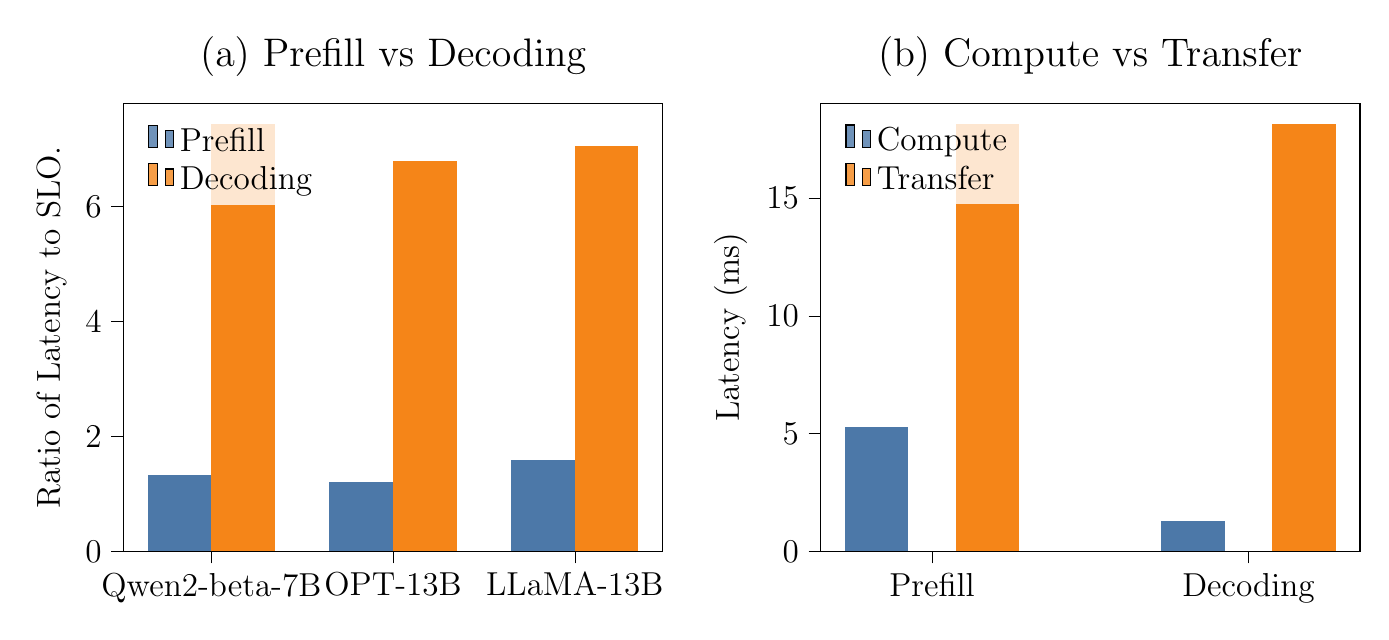
\begin{tikzpicture}

  \definecolor{darkgray176}{RGB}{176,176,176}
  \definecolor{darkorange24513324}{RGB}{245,133,24}
  \definecolor{steelblue76120168}{RGB}{76,120,168}
  
  \begin{groupplot}[group style={group size=2 by 1, horizontal sep=2cm},
    title style={font=\Large},
    label style={font=\large},
    tick label style={font=\large},
    legend style={font=\large}]
  \nextgroupplot[
  legend cell align={left},
  legend style={
    fill opacity=0.8,
    draw opacity=1,
    text opacity=1,
    at={(0.03,0.97)},
    anchor=north west,
    draw=none
  },
  tick align=outside,
  tick pos=left,
  title={(a) Prefill vs Decoding},
  x grid style={darkgray176},
  xmin=-0.485, xmax=2.485,
  xtick style={color=black},
  xtick={0,1,2},
  xticklabels={Qwen2-beta-7B,OPT-13B,LLaMA-13B},
  y grid style={darkgray176},
  ylabel={Ratio of Latency to SLO.},
  ymin=0, ymax=7.8015,
  ytick style={color=black}
  ]
  \draw[draw=none,fill=steelblue76120168] (axis cs:-0.35,0) rectangle (axis cs:0,1.33);
  \addlegendimage{ybar,ybar legend,draw=none,fill=steelblue76120168}
  \addlegendentry{Prefill}
  
  \draw[draw=none,fill=steelblue76120168] (axis cs:0.65,0) rectangle (axis cs:1,1.2);
  \draw[draw=none,fill=steelblue76120168] (axis cs:1.65,0) rectangle (axis cs:2,1.59);
  \draw[draw=none,fill=darkorange24513324] (axis cs:2.77555756156289e-17,0) rectangle (axis cs:0.35,7.43);
  \addlegendimage{ybar,ybar legend,draw=none,fill=darkorange24513324}
  \addlegendentry{Decoding}
  
  \draw[draw=none,fill=darkorange24513324] (axis cs:1,0) rectangle (axis cs:1.35,6.8);
  \draw[draw=none,fill=darkorange24513324] (axis cs:2,0) rectangle (axis cs:2.35,7.06);
  
  \nextgroupplot[
  legend cell align={left},
  legend style={
    fill opacity=0.8,
    draw opacity=1,
    text opacity=1,
    at={(0.03,0.97)},
    anchor=north west,
    draw=none
  },
  tick align=outside,
  tick pos=left,
  title={(b) Compute vs Transfer },
  x grid style={darkgray176},
  xmin=-0.3525, xmax=1.3525,
  xtick style={color=black},
  xtick={0,1},
  xticklabels={Prefill,Decoding},
  y grid style={darkgray176},
  ylabel={Latency (ms)},
  ymin=0, ymax=19.0344,
  ytick style={color=black}
  ]
  \draw[draw=none,fill=steelblue76120168] (axis cs:-0.275,0) rectangle (axis cs:-0.075,5.268);
  \addlegendimage{ybar,ybar legend,draw=none,fill=steelblue76120168}
  \addlegendentry{Compute}
  
  \draw[draw=none,fill=steelblue76120168] (axis cs:0.725,0) rectangle (axis cs:0.925,1.312);
  \draw[draw=none,fill=darkorange24513324] (axis cs:0.075,0) rectangle (axis cs:0.275,18.128);
  \addlegendimage{ybar,ybar legend,draw=none,fill=darkorange24513324}
  \addlegendentry{Transfer}
  
  \draw[draw=none,fill=darkorange24513324] (axis cs:1.075,0) rectangle (axis cs:1.275,18.128);
  \end{groupplot}
  
  \end{tikzpicture}
   % 插入 TikZ 图
 }
    \caption{(a) Serving latency (normalized by the target SLO) with \deepspeed.  
 (b) The average computation and transfer time for a single layer. 
 Model: Qwen2-beta-7B, sequence length: 256, batch size: 4. 
 }
    \label{fig:moti1}
\end{figure}

\begin{figure}[t]
    \centering
    \resizebox{0.6\columnwidth}{!}{
        % This file was created with tikzplotlib v0.10.1.
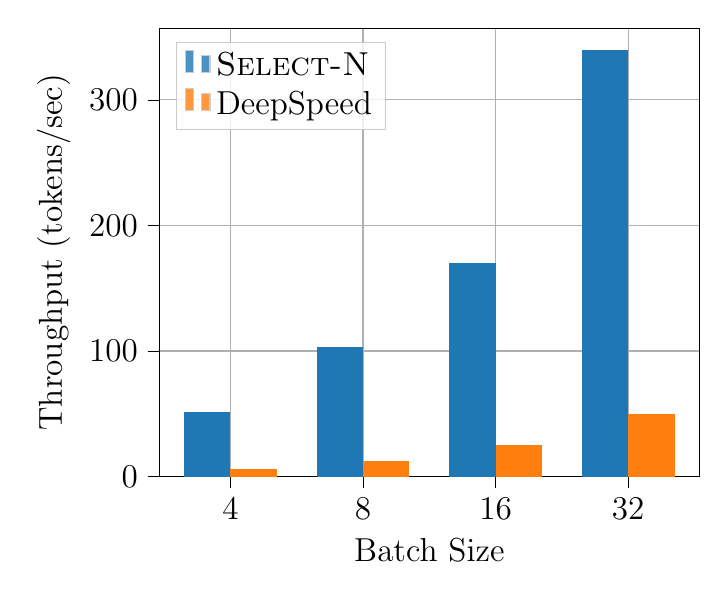
\begin{tikzpicture}

  \definecolor{darkgray176}{RGB}{176,176,176}
  \definecolor{darkorange25512714}{RGB}{255,127,14}
  \definecolor{lightgray204}{RGB}{204,204,204}
  \definecolor{steelblue31119180}{RGB}{31,119,180}
  
  \begin{axis}[
    title style={font=\Large},
    label style={font=\large},
    tick label style={font=\large},
    legend style={font=\large},
  legend cell align={left},
  legend style={
    fill opacity=0.8,
    draw opacity=1,
    text opacity=1,
    at={(0.03,0.97)},
    anchor=north west,
    draw=lightgray204
  },
  tick align=outside,
  tick pos=left,
  % title={Throughput Comparison: \sys vs DeepSpeed},
  x grid style={darkgray176},
  xlabel={Batch Size},
  xmajorgrids,
  xmin=-0.36, xmax=3.71,
  xtick style={color=black},
  xtick={0.175,1.175,2.175,3.175},
  xticklabels={4,8,16,32},
  y grid style={darkgray176},
  ylabel={Throughput (tokens/sec)},
  ymajorgrids,
  ymin=0, ymax=357,
  ytick style={color=black}
  ]
  \draw[draw=none,fill=steelblue31119180] (axis cs:-0.175,0) rectangle (axis cs:0.175,51.54);
  \addlegendimage{ybar,ybar legend,draw=none,fill=steelblue31119180}
  \addlegendentry{\sys}
  
  \draw[draw=none,fill=steelblue31119180] (axis cs:0.825,0) rectangle (axis cs:1.175,103);
  \draw[draw=none,fill=steelblue31119180] (axis cs:1.825,0) rectangle (axis cs:2.175,170);
  \draw[draw=none,fill=steelblue31119180] (axis cs:2.825,0) rectangle (axis cs:3.175,340);
  \draw[draw=none,fill=darkorange25512714] (axis cs:0.175,0) rectangle (axis cs:0.525,6.26);
  \addlegendimage{ybar,ybar legend,draw=none,fill=darkorange25512714}
  \addlegendentry{DeepSpeed}
  
  \draw[draw=none,fill=darkorange25512714] (axis cs:1.175,0) rectangle (axis cs:1.525,12.52);
  \draw[draw=none,fill=darkorange25512714] (axis cs:2.175,0) rectangle (axis cs:2.525,25);
  \draw[draw=none,fill=darkorange25512714] (axis cs:3.175,0) rectangle (axis cs:3.525,50);
  \end{axis}
  
  \end{tikzpicture}
   % 插入 TikZ 图
 }
    \caption{Throughput of \sys and \deepspeed with varying batch sizes. Model: Qwen2-beta-7B}
    \label{fig:moti1c}
\end{figure}


Unfortunately, for most modern LLMs, the computation 
is much shorter than the transfer time of a layer. 
%
We demonstrate this in Figure~\ref{fig:moti1} (b), where the transfer time is 3.5\X and 13.8\X longer than the computation time for the prefill and decoding phase, respectively. 
%
As a result, as shown in Figure~\ref{fig:moti1} (a), \deepspeed increases the
serving latency by up to 9.5\X, resulting in frequent SLO violations for all evaluated models. 
%
In addition to latency, since the GPU waits for the data most of the time, 
such an approach also reduces throughput by up to 8.2\X, as shown in Figure~\ref{fig:moti1c}. 

This is a major limitation since, for many user-facing LLM tasks, such as those discussed in \S\ref{sec:slo}, meeting the latency SLO is the top priority. 
%
Even a single SLO violation incurs a severe economic loss, thus defeating the purpose of minimizing operational costs in offloading approaches. 
%
Therefore, \deepspeed is limited to only those LLM tasks that do not require human interactions. 


\noindent \textbf{Obvervation \#1: Keeping only one layer in GPU, as done by \deepspeed, 
is prone to severe SLO violations.}




%-------------------------------------------------------------------------------

\subsection{Estimating Execution Time}
\label{sec:estimating}



As discussed in \S\ref{sec:prior}, the optimization goal of \flexgen is to 
maximize serving throughput. 
%
To evaluate \flexgen in our target scenario, we made a slight modification to 
the decision algorithm in \flexgen: it now takes a target SLO as input 
and output maximum offloaded portion. 
%
We verify that this modified, SLO-aware version of \flexgen functions correctly and can successfully meet the specified SLOs. 
%
For simplicity, we uses \flexgen to refer to this modified version throughout the rest of the paper. 

We found that a fundamental limitation of \flexgen is that it decides 
the offloaded portion~(\S\ref{sec:prior}) statically~(before 
the requests are actually executed); 
in other words, \flexgen cannot adjust the offloaded portion during execution based on current system status. 
%
Therefore, to avoid SLO violations, with \flexgen, one has to conservatively estimate for the worst case, making \flexgen underutilize host memory but rather uses much more GPU memory than necessary. 
%
As a result, \flexgen often fails to achieve the optimal performance, as shown in Figure~\ref{fig:moti2b}.  
%
The SLO is the TPOT when running without offloading. 
%
In this case, \flexgen uses 2.1\X less host memory than \sys, and thus supports smaller batch sizes, leading to 1.9\X throughput reduction. 
%
We note that this is the best case for \flexgen and a more relaxed SLO 
makes the throughput difference even larger. 

With \flexgen, an important factor for underutilizing host memory is that \flexgen statically estimates serving latency using peak GPU performance. 
%
This is necessary to avoid SLO violations since the estimated value is the theoretical lower bound of the serving latency. 
%
However, as shown in Figure~\ref{fig:moti2}, the estimated latency  
is much shorter than the real one. 
%
This makes \flexgen offload a smaller amount of model state than is necessary to host memory, since \flexgen mistakenly believes that 
the computation time is not long enough to overlap the transfer time of the larger
model state. 

\begin{figure}[t]
    \centering
    \resizebox{\columnwidth}{!}{
        % This file was created with tikzplotlib v0.10.1.
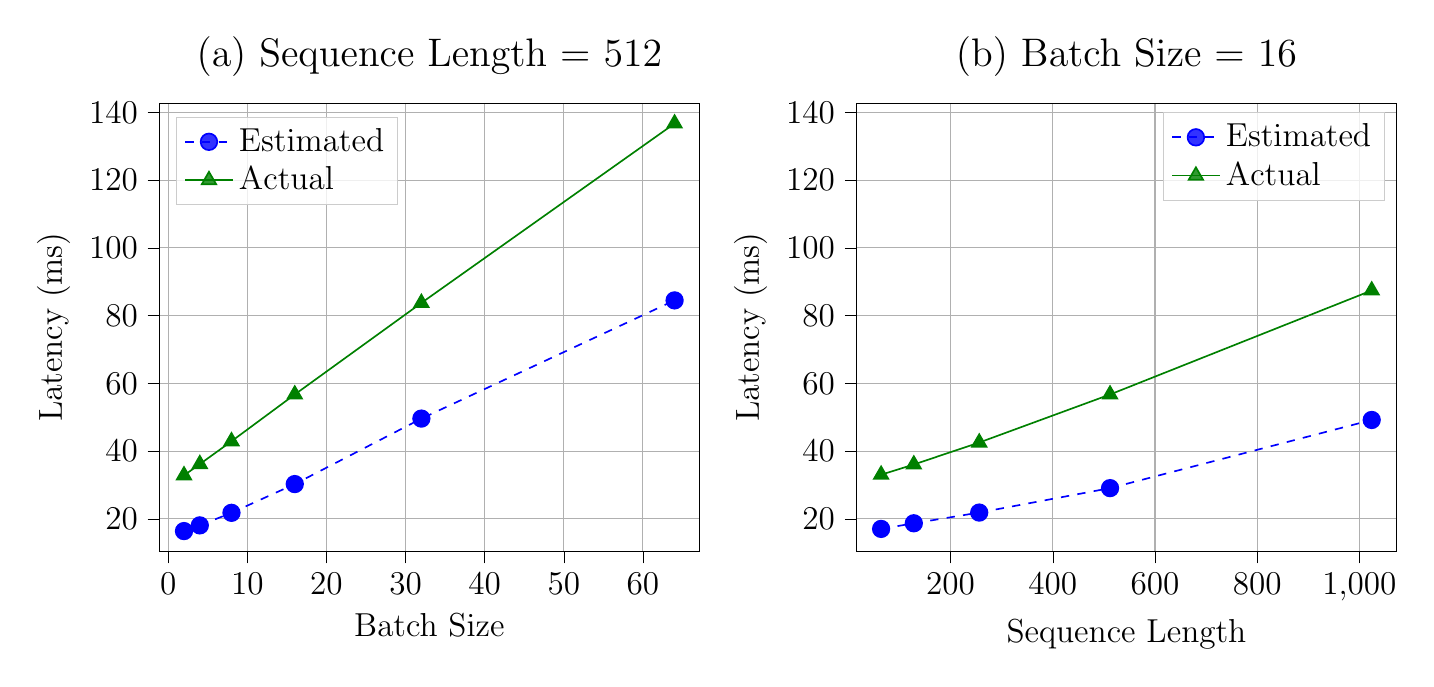
\begin{tikzpicture}

    \definecolor{darkgray176}{RGB}{176,176,176}
    \definecolor{green}{RGB}{0,128,0}
    \definecolor{lightgray204}{RGB}{204,204,204}
    
    \begin{groupplot}[group style={group size=2 by 1, horizontal sep=2cm},
      title style={font=\Large},
    label style={font=\large},
    tick label style={font=\large},
    legend style={font=\large}]
      \nextgroupplot[
        legend cell align={left},
        legend style={
          fill opacity=0.8,
          draw opacity=1,
          text opacity=1,
          at={(0.03,0.97)},
          anchor=north west,
          draw=lightgray204
        },
        tick align=outside,
        tick pos=left,
        title={(a) Sequence Length = 512},
        x grid style={darkgray176},
        xlabel={Batch Size},
        xmajorgrids,
        xmin=-1.1, xmax=67.1,
        xtick style={color=black},
        y grid style={darkgray176},
        ylabel={Latency (ms)},
        ymajorgrids,
        ymin=10.3955, ymax=142.7145,
        ytick style={color=black}
        ]
        \addplot [semithick, blue, dashed, mark=*, mark size=3, mark options={solid}]
        table {%
        2 16.41
        4 18.091
        8 21.79
        16 30.277
        32 49.604
        64 84.493
        };
        \addlegendentry{Estimated}
        \addplot [semithick, green, mark=triangle*, mark size=3, mark options={solid}]
        table {%
        2 32.85
        4 36.17
        8 42.91
        16 56.72
        32 83.74
        64 136.7
        };
        \addlegendentry{Actual}
        
        \nextgroupplot[
        legend cell align={left},
        legend style={fill opacity=0.8, draw opacity=1, text opacity=1, draw=lightgray204},
        scaled y ticks=manual:{}{\pgfmathparse{#1}},
        tick align=outside,
        tick pos=left,
        title={(b) Batch Size = 16},
        x grid style={darkgray176},
        xlabel={Sequence Length},
        xmajorgrids,
        xmin=16, xmax=1072,
        xtick style={color=black},
        y grid style={darkgray176},
        ylabel={Latency (ms)},
        ymajorgrids,
        ymin=10.3955, ymax=142.7145,
        ytick style={color=black},
        ]
        \addplot [semithick, blue, dashed, mark=*, mark size=3, mark options={solid}]
        table {%
        64 17.043
        128 18.709
        256 21.87
        512 29.08
        1024 49.196
        };
        \addlegendentry{Estimated}
        \addplot [semithick, green, mark=triangle*, mark size=3, mark options={solid}]
        table {%
        64 33.04
        128 36.06
        256 42.54
        512 56.72
        1024 87.42
        };
        \addlegendentry{Actual}
        \end{groupplot}
        
        \end{tikzpicture}
         % 插入 TikZ 图
 }
    \caption{The actual serving latency vs. the one estimated by \flexgen. Model: OPT-13B.
 }
    \label{fig:moti2}
\end{figure}

\begin{figure}[t]
    \centering
    \resizebox{\columnwidth}{!}{
        % This file was created with tikzplotlib v0.10.1.
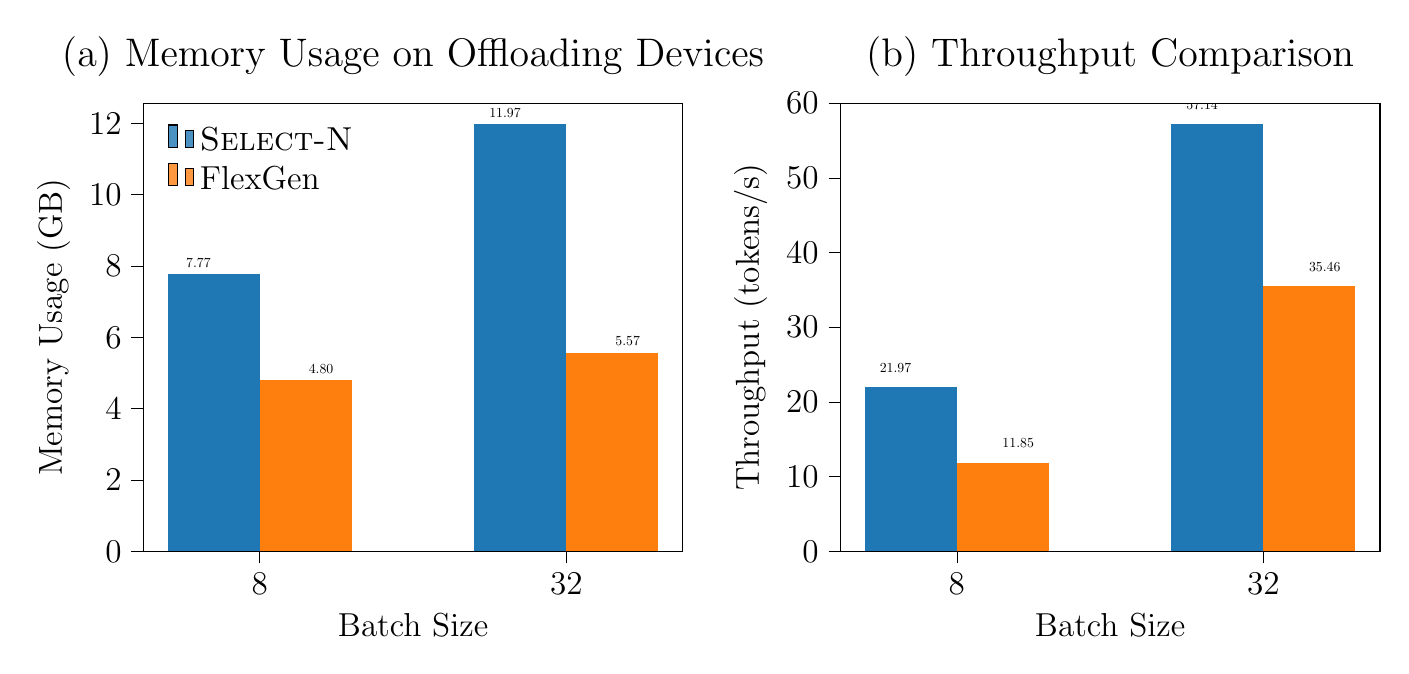
\begin{tikzpicture}

  \definecolor{darkgray176}{RGB}{176,176,176}
  \definecolor{darkorange25512714}{RGB}{255,127,14}
  \definecolor{steelblue31119180}{RGB}{31,119,180}
  
  \begin{groupplot}[group style={group size=2 by 1, horizontal sep=2cm},
    title style={font=\Large},
    label style={font=\large},
    tick label style={font=\large},
    legend style={font=\large}]
  \nextgroupplot[
  legend cell align={left},
  legend style={
    fill opacity=0.8,
    draw opacity=1,
    text opacity=1,
    at={(0.03,0.97)},
    anchor=north west,
    draw=none
  },
  tick align=outside,
  tick pos=left,
  title={(a) Memory Usage on Offloading Devices},
  x grid style={darkgray176},
  xlabel={Batch Size},
  xmin=-0.38, xmax=1.38,
  xtick style={color=black},
  xtick={0,1},
  xticklabels={8,32},
  y grid style={darkgray176},
  ylabel={Memory Usage (GB)},
  ymin=0, ymax=12.5685,
  ytick style={color=black}
  ]
  \draw[draw=none,fill=steelblue31119180] (axis cs:-0.3,0) rectangle (axis cs:0,7.77);
  \addlegendimage{ybar,ybar legend,draw=none,fill=steelblue31119180}
  \addlegendentry{\sys}
  
  \draw[draw=none,fill=steelblue31119180] (axis cs:0.7,0) rectangle (axis cs:1,11.97);
  \draw[draw=none,fill=darkorange25512714] (axis cs:2.77555756156289e-17,0) rectangle (axis cs:0.3,4.8);
  \addlegendimage{ybar,ybar legend,draw=none,fill=darkorange25512714}
  \addlegendentry{FlexGen}
  
  \draw[draw=none,fill=darkorange25512714] (axis cs:1,0) rectangle (axis cs:1.3,5.57);
  \draw (axis cs:-0.2,7.97) node[
    scale=0.5,
    anchor=base,
    text=black,
    rotate=0.0
  ]{7.77};
  \draw (axis cs:0.8,12.17) node[
    scale=0.5,
    anchor=base,
    text=black,
    rotate=0.0
  ]{11.97};
  \draw (axis cs:0.2,5) node[
    scale=0.5,
    anchor=base,
    text=black,
    rotate=0.0
  ]{4.80};
  \draw (axis cs:1.2,5.77) node[
    scale=0.5,
    anchor=base,
    text=black,
    rotate=0.0
  ]{5.57};
  
  \nextgroupplot[
  legend cell align={left},
  legend style={
    fill opacity=0.8,
    draw opacity=1,
    text opacity=1,
    at={(0.03,0.97)},
    anchor=north west,
    draw=none
  },
  tick align=outside,
  tick pos=left,
  title={(b) Throughput Comparison},
  x grid style={darkgray176},
  xlabel={Batch Size},
  xmin=-0.38, xmax=1.38,
  xtick style={color=black},
  xtick={0,1},
  xticklabels={8,32},
  y grid style={darkgray176},
  ylabel={Throughput (tokens/s)},
  ymin=0, ymax=59.997,
  ytick style={color=black}
  ]
  \draw[draw=none,fill=steelblue31119180] (axis cs:-0.3,0) rectangle (axis cs:0,21.97);
  \draw[draw=none,fill=steelblue31119180] (axis cs:0.7,0) rectangle (axis cs:1,57.14);
  \draw[draw=none,fill=darkorange25512714] (axis cs:2.77555756156289e-17,0) rectangle (axis cs:0.3,11.85);
  \draw[draw=none,fill=darkorange25512714] (axis cs:1,0) rectangle (axis cs:1.3,35.46);
  \draw (axis cs:-0.2,23.97) node[
    scale=0.5,
    anchor=base,
    text=black,
    rotate=0.0
  ]{21.97};
  \draw (axis cs:0.8,59.14) node[
    scale=0.5,
    anchor=base,
    text=black,
    rotate=0.0
  ]{57.14};
  \draw (axis cs:0.2,13.85) node[
    scale=0.5,
    anchor=base,
    text=black,
    rotate=0.0
  ]{11.85};
  \draw (axis cs:1.2,37.46) node[
    scale=0.5,
    anchor=base,
    text=black,
    rotate=0.0
  ]{35.46};
  \end{groupplot}
  
  \end{tikzpicture}
   % 插入 TikZ 图
 }
    \caption{Comparison of \sys and FlexGen in (a) Memory usage on the offloading devices and (b) Throughput. Model: OPT-13B.}
    \label{fig:moti2b}
\end{figure}



\noindent \textbf{Obvervation \#2: Estimating model execution time 
using peak GPU performance, as with \deepspeed, is inaccurate and 
heavily underutilizes host memory.}



%-------------------------------------------------------------------------------

\subsection{Bandwidth Contention}
\label{sec:bandwidth}

Another important factor for \flexgen to underutilize host memory is 
the contention on transfer bandwidth between host and GPU memory. 
%
Specifically, to minimize operational costs, the current industry practice is to place multiple GPUs on a single machine node. 
%a
However, some of these GPUs share a single PCIe bus~(which connects the host and GPUs), and thus contends for the PCIe bandwidth~\cite{pciecontention, pciecontention2}. 
% cite some papers on the PCIe contention caused by GPUs. 
%
As a result, the available bandwidth to transfer LLM state for each 
individual GPU fluctuates during serving a request. 

With \flexgen, in the presence of bandwidth contention, to meet SLO, 
one must again estimate the worst case:  
%
each GPU only gets $1/n$ of the bandwidth, where $n$ is the number of GPUs that share a PCIe bus.  
%
However, for a given GPU, the available bandwidth may fluctuate but is often much larger than the worst-case one, since other GPUs may be idle, or do not 
fully utilize their share of the bandwidth. 
%
As a result, \flexgen overestimates the transfer time, again offloading a smaller amount of LLM state than is necessary to host memory. 



\noindent \textbf{Observation \#3: \flexgen statically estimates the PCIe bandwidth under contention, thereby underutilizing the host memory.}


%-------------------------------------------------------------------------------
\section{The \sys System}
%-------------------------------------------------------------------------------

This section presents \sys, an latency-SLO-aware memory offloading 
system for LLM inference. 
%
This section starts with \syss design goals~(\S\ref{sec:designgoals}), an overview~(\S\ref{sec:overview}), followed by the design of each  component.

\subsection{Design Goals.}
\label{sec:designgoals}
%
We design \sys with the following goals. 

\squishlist
%
\item{\textbf{Meeting latency SLOs.}}
%
Departing from \deepspeed, the top priority of \sys is to meet latency SLOs, aligning with the overarching goal of memory offloading: reducing operational costs. 

\item{\textbf{Maximizing host memory usage.}}
%
Once adhering to latency SLO, unlike \flexgen, \sys should maximize host memory usage to \eg, support larger models, enable greater batch sizes and/or longer sequence lengths, or allow the models to produce longer outputs. 

\item{\textbf{Fine-grained dynamic adjusting.}}
%
\sys should dynamically (rather than statically as with \flexgen) decide the amount of memory offloaded to the host, considering factors such as the sequence length and batch size of serving requests, the associated latency SLOs and, particularly, the current machine status.
\squishend

\subsection{Overview}
\label{sec:overview}
%-----------------------------------

\PN{Deployment scenario.} 
%
\sys operates on a single machine equipped with multiple GPUs, where each hosts a model. 
%
These GPUs may contend on the PCIe bandwidth. 
%
\sys takes as input a serving request and its associated SLO. 
%
Such an SLO may not be the end-to-end one: upper level components can adjust the SLO passed to \sys based on, \eg, networking delays that are 
already incurred. 
%
\sys next checks whether this SLO can be met by the GPUs it 
manages~(\S\ref{subsec:des:contention}), as there are situations where 
the SLO cannot be met at all. 
%
For example, a deployed model with weights requiring memory far exceeding the GPU's capacity forces a large state to be offloaded to host memory, 
causing long data transfer times that violate the SLO. 
%
If the SLO can be met, \sys schedules the request on one of the GPUs. 
%
If not, \sys passes the request to the upper-level scheduler, which can 
avoid the SLO violation, by, \eg, sending the requests to other node hosting
models without memory offloading. 
%

%
\PN{Components and workflow.}
%
To meet the design goals, at its core, \sys operates on the \interval~(\S\ref{sec:runtimememorymanager}), 
an internal tunable knob that captures the tradeoff between 
meeting SLOs and maximizing host memory usage. 
%
A small \interval makes \sys offload more LLM state to host memory and thus 
may potentially slow down inference, being more prone to SLO violations.  
%
A large \interval achieves the opposite. 
%
As further explained in \S\ref{sec:runtimememorymanager}, using \interval to control 
the aforementioned tradeoff is enabled by a unique characteristic of LLM: 
during serving, each layer takes the same amount of computation time. 
%
Thanks to \interval, meeting the design goals of \sys is reduced to automatically and dynamically adjusting the \interval for each GPU instance. 
%
\sys achieves this in two stages: first an offline stage and then 
an online stage, as we detail next. 

As shown in Figure~\ref{fig:overview}, \sys consists of three components: 1) a performance 
\analyzer, to find the optimal \interval~(\ie, the smallest one that meets SLO) under no bandwidth contention; 2) per-GPU runtime memory 
managers, which take as input \interval, and transfers layer state between GPU 
and host memory basd on the \interval; and 3) per-bus runtime 
bandwidth coordinators, which adjust the \interval for all GPUs 
sharing a bus at the granularity of each inference iteration. 
%

The performance \analyzer operates offline~(\ie, not on servers that handle user requests) to find the optimal \interval.
%
Specifically, to ensure no bandwidth contention, the performance 
\analyzer operates on a dedicated server,
where each GPU exclusively occupies a single PCIe bus.
%
Upon deploying a new model on a GPU that \sys manages, the model is passed to the performance \analyzer. 
%
The \analyzer generates a stream
of prompts and executes them on the model to generate a performance \record. 
%
A performance \record stores the optimal \interval for all valid combinations of SLOs, sequence length, and batch size. 
%
Generating a performance \record beforehand is possible due to, again, LLM's deterministic execution time. 
%
Unlike performance \analyzer, the memory manager and bandwidth coordinators operate online on normal servers that serve user requests. 



The workflow of \sys is as follows.
%
When a request comes,
\BC{1}
%
\sys first waits for a GPU instance hosting the corresponding model to become available.
%
\BC{2}
%
Based on the target SLO~(minus the waiting time), the 
sequence length, and the batch sizes of the request, 
\sys consults the performance \record of the model to obtain the optimal
\interval. 
%
\BC{3} 
%
The \interval and the requests are passed to the bandwidth coordinator, which 
generates an adjusted \interval for each GPU instance that shares the bus considering their bandwidth utilization. 
%
\BC{4} 
%
The bandwidth coordinator passes the request to the selected GPU, and the 
set of adjusted \interval to the runtime memory managers of all GPUs sharing the bus. 
%
The runtime memory manages applies the adjusted \interval before the next inference iteration. 
%


%---------------------------
\begin{figure}[t]
    \centering
    \includegraphics[width=\columnwidth]{figures/overview.pdf}
    \caption{The architecture and workflow of \sys.}
    \label{fig:overview}
\end{figure}

%% %---------------------------


\subsection{Runtime Memory Manager}
\label{sec:runtimememorymanager}
%
\PN{Insight.}
%
A key design behind \interval is to exploit a special characteristic of LLM:  during inference, the computation time of each layer is always identical, even in different iterations.
%
This is because, as discussed in \S\ref{sec:llm}, 1) each layer consists of the 
same structure~(\ie, same number of matrices of the same size for the corresponding matrices); 
%
2) each layer performs the same operations, 
%
and 3) the size of the input to each layer remains the same~(\ie, either all 
input tokens in prefill or one token in decoding). 
%


\PN{\Interval.}
%
Using this, \sys proposes \interval. 
%
An \interval of $i$ means that for every $i$ layer, the state of the last layer is offloaded to CPU memory, while the state of other layers are always 
in GPU memory. 
%
We term the last layer \oflayer. 
%

The memory manager in \sys transfers the state between host and GPU memory following a decided \interval. 
%
To maximize performance, \sys also follows the design scheme of overlapping computation with data transfer~(\S\ref{sec:overview}). 
%
However, unlike \deepspeed and \flexgen that prefetches the \oflayer only when 
the computation is on the exact previous layer, the memory manager in \sys prefetches the state of the \oflayer by initiating the loading upon the computation on the first layer 
in the \interval.  
%
Therefore, with \sys, 
the transfer time is hidden by the computation time of multiple layers, rather than one layer as \deepspeed and \flexgen. 


%---------------------------
\begin{figure*}[t]
    \centering
    \includegraphics[width=\textwidth]{figures/overlap.pdf}
    \caption{An overview of how a memory manager works. 
 The upper part represents the compute stream, where each block denotes 
 a layer with pink blocks being the offloaded layers. 
    %
 The lower part is the copy stream. 
 The two streams execute in parallel, with "S" meaning synchronization points between the streams.}
    \label{fig:selectn}
\end{figure*}

%% %---------------------------

Figure~\ref{fig:selectn} concretizes the above discussion by showing a scenario where the \interval is 4. 
%
In this case, the states of layers 1 to 3 and 5 to 7 are always in the GPU memory, while layers 4 and 8 are \oflayer. 
%
Before computing layers 1 and 5, \sys prefetches the state of layers 4 and 8, respectively. 
%
Next, before computing layers 4 and 8, \sys ensures that their state 
is ready in the GPU memory. 
%
Once the computation is done, \sys moves their state back to CPU. 

The \interval offers an effective mechanism to resolve the tension between meeting the SLO and maximizing host memory usage. 
%
A small \interval maximizes host memory usage, since more layers are offloaded there, but can only support looser SLO, since there are fewer layers 
whose computations are used to hide the load of the \oflayer. 
%
In fact, \sys is reduced to \deepspeed if the \interval is set to $1$. 
%
A larger \interval increases GPU memory usages, but can meet stricter SLO. 
%

The above design simplifies resolving the aforementioned tension to 
selecting an optimal (\ie, the smallest \interval that meets the SLO of given input requests). 
%
The following subsections present how \sys performs the selection with a 
two-phase approach. 

\subsection{Generating Performance \Record}
\label{sec:generatingperformance}
%-------------------------------------------------------------------------------

\PN{Challenge.}
%
To decide the optimal \interval, one must know the computation time and the transfer time of each layer. 
%
A challenge \sys encounters is that while the computation time of each layer 
is highly deterministic~(\ie, the time is always the same), it is not
predictable; one cannot easily estimate beforehand the computation time 
of each layer, as we have shown in~\S\ref{sec:estimating}. 
%
As a result, this forces \sys to measure this computation time during runtime. 
%
An naive approach is to measure the computation time on the real production server every time the actual requests arrive. 
%
However, this 1) increases GPU usage, thereby 
leading to extra operational costs; 2) incurs an extra latency caused by 
measurements during runtime. 


\begin{table}[t]
    \centering
    \small % 使用较小的字体
    \begin{tabular}{c|cccc}
        \hline
        \textbf{} & \textbf{128} & \textbf{256} & \textbf{512} & \textbf{1024} \\ \hline
        \textbf{4}   & 5 & 4 & 3 & 2 \\
        \textbf{8}   & 4 & 3 & 2 & 1 \\
        \textbf{16}  & 3 & 2 & 1 & 1 \\
        \textbf{32}  & 2 & 1 & 1 & 1 \\
        \textbf{64}  & 1 & 1 & 1 & 1 \\  \hline
        % \textbf{128} & 1 & 1 & 1 & 1 \\ \hline
    \end{tabular}
    \vspace{0.6cm}
    \caption{Performance \record for a given SLO. 
 Row: batch size. Column: sequence length. Larger batch sizes and sequence lengths are omitted, as the optimal \interval is one.}
    \label{tab:batchtpotdecode}
\end{table}



\PN{Insight.}
%
\sys overcomes this challenge, again by leveraging the deterministic nature of the computation time on each layer.
%
Our obsveration is that, with the deterministic nature, for a given model and hardware platform, assuming no bandwidth contention, 
the computation time of each layer depends solely on 
the size of the prompts, namely the sequence length and batch size.  
%
Therefore, \sys can obtain the accurate execution time of each layer 
by simply executing one iteration of the model on the target machine.  
%  


\PN{Design.}
%
The above insight allowed \sys to decide the optimal \interval offline with 
a model \analyzer. 
%
The \analyzer is invoked every time a new model is scheduled to 
be deployed on a GPU instance managed by \sys. 
%
The \analyzer takes as input a list of potentially possible SLOs, 
and for each SLO, generates a performance \record. 
%
The performance \record stores, for a pair of input sequences and batch size, 
the optimal \interval, assuming no bandwidth contention. 
%
Table~\ref{tab:batchtpotdecode} shows one such example. 

Under the hood, the \analyzer works in the following steps. 
%
For a given SLO, it first enumerates all possible pairs of batch size and sequence length. 
%
For any given pair, the \analyzer generates a prompt of that size with 
random content. 
%
It next uses the prompt to run one iteration of prefill and decoding. 
%
During execution, the \analyzer measures 1) $t_\text{trans}$: 
the time to transfer a layer from CPU to GPU memory; 2) 
and then $t_\text{compute}$: the computation time of a single layer. 
%
Therefore, to ensure the layer transferring time does not cause SLO violations, 
the maximum number of layers that can be offloaded 
is $L_{\text{offload}} = \left\lfloor \frac{t_\text{compute} \cdot (1 + \delta)}{t_\text{trans}} \right\rfloor$, where $\delta$ is the SLO quotient
over the computation time without offloading. 
%
Finally, the optimal \interval for this pair of sequence length and batch size is given by \(\left\lfloor \frac{L}{L_{\text{offload}}} \right\rfloor\), 
where \(L\) is the total number of decoder layers in the model.




Creating performance \records is practical for the following reasons. 
%
First, the number of combinations of batch size, sequence length, and SLOs that need to be enumerated is actually small, since the \analyzer only needs to operate at a specific granularity for these values to be effective.
%
For example, the current prototype uses 2-millisecond granularity for SLOs and requires batch sizes and sequence lengths to be powers of two.
%
\sys selects the optimal offloading interval for combinations not listed in the performance record by conservatively choosing from the nearest combination.
%
With this granularity, the number of target SLOs in production is typically 
at the scale of hundreds, since latency SLOs for interactive LLM tasks, which
sys targets, rarely exceed one second.
% 
Although there can be an infinite number of batch size and sequence length pairs, if their product exceeds a certain threshold, the optimal \interval becomes 1, since the computational time of a single layer exceeds the 
transfer time of that layer.  
%
Therefore, the possible pairs of the batch size and sequence length the \analyzer needs to sample is at most 100 for our evaluated models.  
%
Second, given a batch size and sequence length pair, obtaining the optimal
\interval is fast, which usually takes 1-2 seconds for our models. 
%
The above two factors combined mean that the process of creating a performance \record is fast, requiring at most 40 minutes for our models. 
%
This is much shorter than the frequency of deploying a new model in production, 
which is at the scale of months. 


\PN{Supporting the separation of prefill and decoding.}
%
An emerging LLM deployment scheme is to deploy prefill and decoding phases on separate instances~\cite{distserve, splitwise}. 
%
Such separation maximizes performance by allowing each stage to 
fully leverage GPUs optimized for their specific workloads. 
%
In addition, the separation facilitates independent scaling of the two phases. 

Unfortunately, both \deepspeed and \flexgen do not consider the separation
of prefill and decoding; 
%
they offload the same portion of the model state to host memory for both phases, 
thereby causing significantly longer delays during the decoding phase. 


A key benefit enabled by the \analyzer is to effectively support the seperation of prefill and decoding.   
%
In this case, the \analyzer creates the performance \record for prefill and decoding separately, thereby considering the different characteristics of the two phases. 
%
Hence, departing from prior work, \sys can use a different \interval that is most suitable for the corresponding phase. 
%
In general, the compute-intensive prefill phase requires a shorter \interval, 
while the memory-intensive decoding phase requires a larger \interval.  
%



%-------------------------------------------------------------------------------
\subsection{Addressing Bandwidth Contention}
\label{subsec:des:contention}

%
The \analyzer chooses the optimal \interval by assuming 
an ideal scenario where each GPU can utilize the whole PCIe bandwidth. 
%
However, as discussed in \S\ref{sec:bandwidth}, real-world inference scenarios may incur bandwidth contention among different GPU instances.  
%
\sys addresses this issue with a per-bus runtime bandwidth coordinator, that adjusts \interval for contented GPU instances at the granularity of each inference iteration~(\ie, at the granularity of generating an output token), as we detail next. 
%

The coordinator performs the adjustment by observing that, given an input request, each GPU instance has a minimum and maximum \interval. 
%
The minimum \interval is derived from the performance \record~(\S\ref{sec:generatingperformance}); 
%
any \interval below the minimum violates the SLO of the input.  
%
The maximum \interval depends on the model memory deployed on the GPU. 
%
Since \sys enables deploying models that require more memory than the GPU has, the 
\interval must remain below a threshold to avoid exceeding GPU capacity. 
%
For models whose required memory is within the GPU capacity, the
maximum \interval is infinite. 

Critically, the \interval also 
precisely controls the usage of PCIe bandwidth. 
%
A small \interval incurs higher bandwidth usage since layers are swapped more frequently between host and GPU memory, while a large \interval incurs lower bandwidth. 
%
Furthermore, given an \interval, the consumed bandwidth can be accurately estimated, as shown in Lines 4-13 of Figure~\ref{fig:code}. 

Therefore, with the above setup, to avoid SLO violations, the coordinator needs 1) to pick, for each contented GPU instance, 
a valid \interval that falls between the minimum and maximum interval; 
%
and 2) ensures that the sum of the PCIe bandwidth consumed for each \interval 
is below the PCIe bandwidth. 
%
In addition, another goal of \sys is to optimize the right set of \interval to maximize the total usage of host memory. 
%
\sys can also adopt other reasonable optimization goals. 
%
For the sake of simplicity, the rest of the discussion assumes two contented 
GPU instances, but the algorithm can be easily extended to more instances. 

\begin{figure}[t]
    \centering
    \includegraphics[width=\columnwidth]{figures/code.png}
    \caption{The adjustment algorithm performed by the coordinator. }
    \label{fig:code}
\end{figure}

%
Figure~\ref{fig:code} shows how the coordinator works. 
%
Upon receiving a new request, the coordinator first checks if this request's SLO can possibly be met by checking if its minimum \interval is less than the maximum one~(Lines 34-35).  
%
If no valid interval can be found, the request is returned to the upper level 
scheduler~(\S\ref{sec:overview}). 
%
Otherwise, the coordinator enumerates all possible combinations of \intervals for the two GPU instances to find all the valid ones~(Lines 39-42). 
%
Next, the coordinator finds the interval pairs that maximize host GPU memory 
usage~(Line 45). 
%
Once the valid interval pairs are decided, the request is served on one GPU 
with the chosen interval while the other GPU adjusts the interval in the next 
iteration~(Lines 47-48). 
%
We note that a special case is that the other GPU is idle, and in this case, 
the request is served with the minimum \interval. 
%

\subsection{Implementation}
%
\sys is implemented based on the vLLM framework, leveraging its efficient memory management and inference capabilities. 
To optimize performance, \sys uses separate CUDA streams for computation and data transmission. 
By enabling parallel execution through stream overlap, \sys significantly reduces latency and improves throughput during inference.

We encapsulated \sys into a Python library that allows seamless integration with Transformer-based models. 
This library dynamically manages the decoder layers of the model, enabling efficient scheduling and resource allocation. 
With this design, users can easily wrap existing Transformer models to take advantage of \sys without requiring extensive modifications while benefiting from enhanced performance and scalability.


%-------------------------------------------------------------------------------
\section{Evaluation}
%-------------------------------------------------------------------------------


\subsection{Experimental Setup}
\label{sec:expsetup}

\PN{Model and System Configuration.} 
The experiments are conducted on a system equipped with 4 NVIDIA A10 GPUs. 
The models used in this study include OPT-6.7B, OPT-13B, Qwen2-beta-7B, and Llama2-13B. 
These models were selected to represent a range of sizes and complexities, ensuring a thorough evaluation of the \sys mechanism on varying model scales. 
Unless otherwise specified, 
all experiments are conducted using a separation of the prefill and decoding phases, with each model deployed as two distinct instances: a prefill instance and a decoding instance.

\PN{Workload.} 
The workload used in the experiments is generated using a randomly designed dataloader, which allows users to customize batch size, sequence length, 
and vocabulary size based on the model requirements. Our setup can equally support real-world workloads, 
such as ShareGPT\cite{sharegpt} and Alpaca\cite{alpaca1, alpaca2} datasets, as the fundamental workload characteristics are consistent and do not significantly impact experimental results.

\PN{Baseline.} 
We consider three baselines in our evaluation: DeepSpeed, FlexGen, and a naive method.
The naive method, built upon the vLLM framework, involves loading the entire model into GPU memory without any offloading. 
Our \sys mechanism is also implemented on top of the vLLM framework, whose paged attention mechanism enables fine-grained memory management during inference.

\PN{Key Metrics.} 
We use several key metrics to evaluate performance, 
including GPU memory savings for memory efficiency, TTFT and TPOT for latency, and throughput for overall inference performance across prefill and decoding phases.


\subsection{Maintaining SLO}

We conduct experiments using the OPT-6.7B model and the Qwen2-beta-7B model with clear separation of the prefill and decoding phases to show the capability of \sys in maintaining SLO. 
The prefill phase corresponds to the TTFT SLO, while the decoding phase corresponds to the TPOT SLO. 
This separation enables us to apply different \interval values to the two instances, allowing each phase to meet its respective SLO effectively.

Due to the benefits of separation, which allows for an increased batch size in the decoding instance as we discussed earlier, we fix the batch size at 128 for the decoding instance and 32 for the prefill instance to simulate a realistic high-throughput inference scenario. 
As a baseline, we measure the performance under a naive execution mode without offloading, where the TTFT and TPOT latencies are recorded as reference points. 
Subsequently, we configured \sys to operate under varying SLO constraints for both TTFT and TPOT to test its ability to meet these requirements by adjusting the \interval parameter. 
Furthermore, we conducted experiments to compare the performance of \sys with DeepSpeed.

To ensure consistency, the SLO values are normalized to 1, 
and the recorded values represent the ratio of the observed time to the specified SLO. 
The results shown in Figure~\ref{fig:eval1} demonstrate that 
\sys effectively maintains the specified SLOs for both TTFT and TPOT in different setups. 
It further illustrates how \sys adapts to varying SLO constraints by dynamically adjusting the \interval parameter. 
When the SLO is set within the range 20\%-40\%,
the optimal \interval remains unchanged, resulting in relatively stable TPOT values. 
As the SLO increases from 40\% to 50\%, 
the optimal \interval selected during the experiment changes, 
causing a noticeable variation in the TPOT curve.

DeepSpeed suffers from significant transmission latency during inference. 
This bottleneck is particularly severe in the decoding phase, where the large volume of parameter transfers drastically amplifies the delay, 
resulting in exceeding the specified SLOs by 8.08\X and reducing its throughput by 6.8\X to 8.23\X compared to \sys.

\begin{figure}[t]
    \centering
    \resizebox{\columnwidth}{!}{
        % This file was created with tikzplotlib v0.10.1.
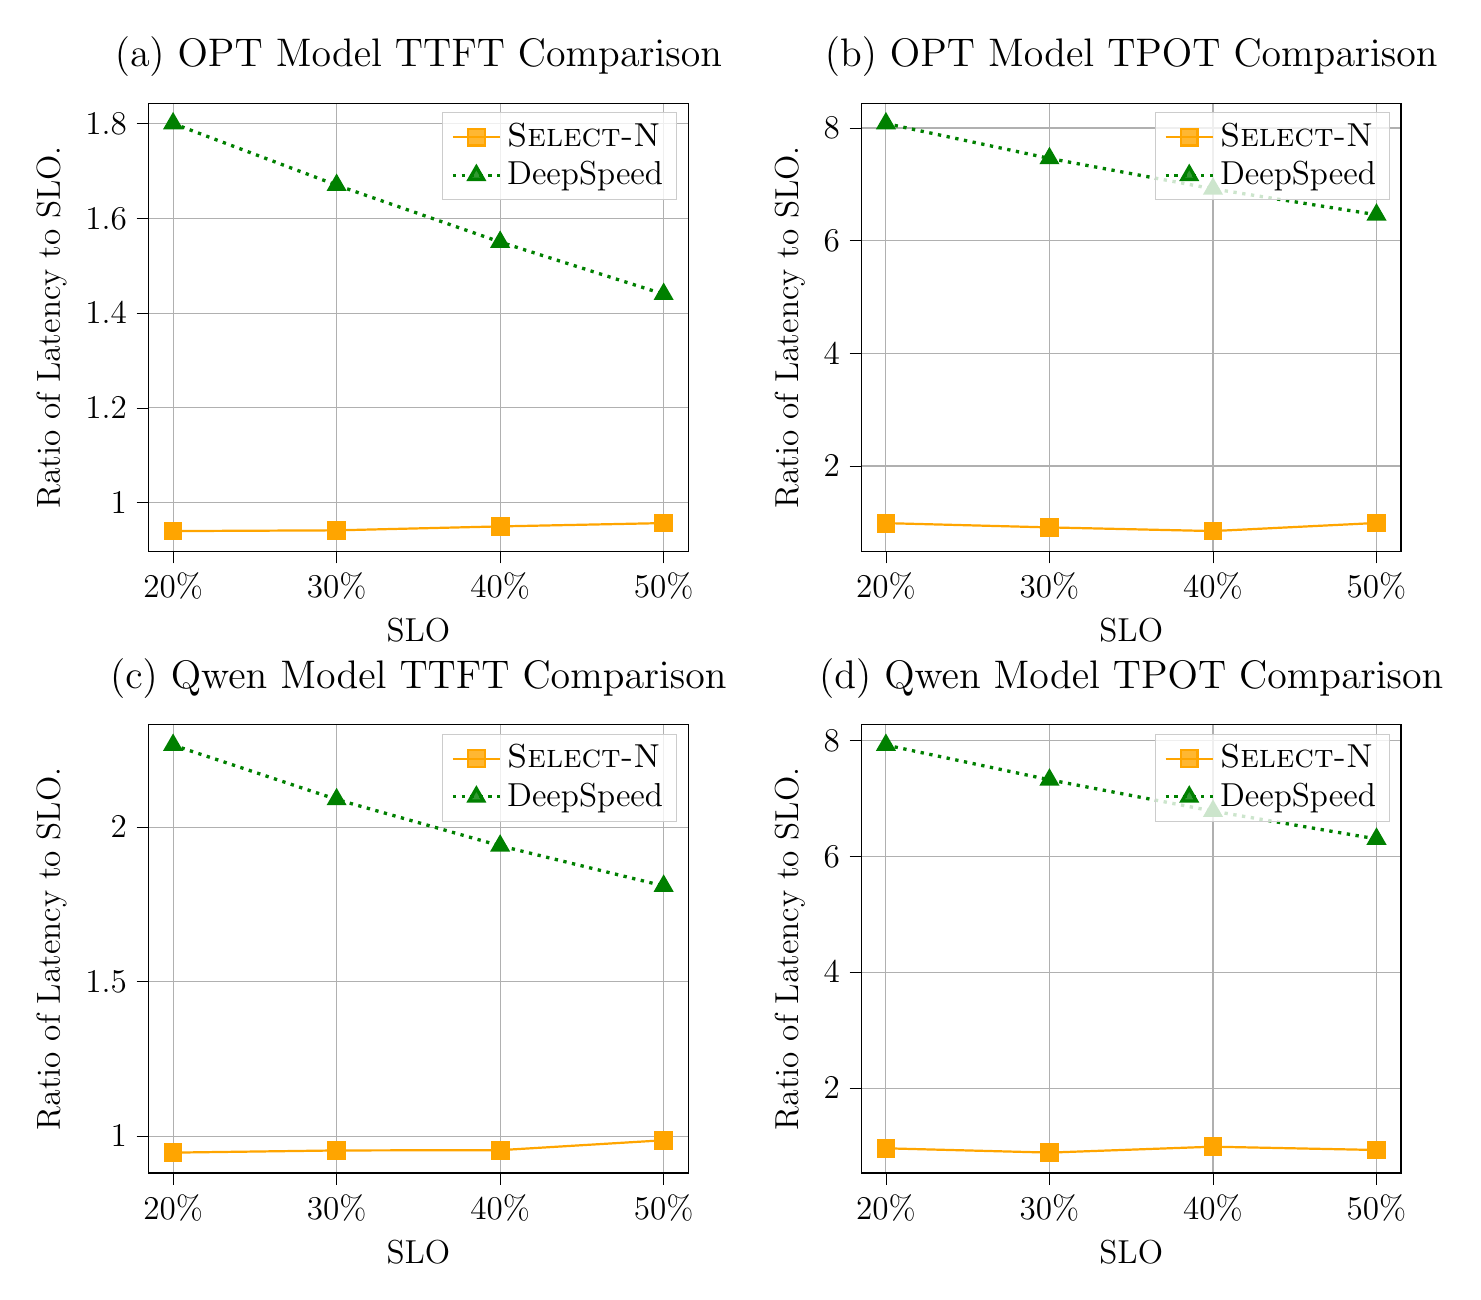
\begin{tikzpicture}

  \definecolor{darkgray176}{RGB}{176,176,176}
  \definecolor{green}{RGB}{0,128,0}
  \definecolor{lightgray204}{RGB}{204,204,204}
  \definecolor{orange}{RGB}{255,165,0}
  
  \begin{groupplot}[group style={group size=2 by 2, horizontal sep=2.2cm, vertical sep=2.2cm},
    title style={font=\Large},
    label style={font=\large},
    tick label style={font=\large},
    legend style={font=\large}]
    \nextgroupplot[
      legend cell align={left},
      legend style={fill opacity=0.8, draw opacity=1, text opacity=1, draw=lightgray204},
      tick align=outside,
      tick pos=left,
      title={(a) OPT Model TTFT Comparison},
      x grid style={darkgray176},
      xlabel={SLO},
      xmajorgrids,
      xmin=-0.15, xmax=3.15,
      xtick style={color=black},
      xtick={0,1,2,3},
      xtick={0,1,2,3},
      xtick={0,1,2,3},
      xticklabels={20\%,30\%,40\%,50\%},
      xticklabels={20\%,30\%,40\%,50\%},
      xticklabels={20\%,30\%,40\%,50\%},
      y grid style={darkgray176},
      ylabel={Ratio of Latency to SLO.},
      ymajorgrids,
      ymin=0.8971575, ymax=1.8429925,
      ytick style={color=black}
      ]
      \addplot [thick, orange, mark=square*, mark size=3, mark options={solid}]
      table {%
      0 0.94015
      1 0.9417
      2 0.95
      3 0.957
      };
      \addlegendentry{\sys}
      \addplot [very thick, green, dotted, mark=triangle*, mark size=3, mark options={solid}]
      table {%
      0 1.8
      1 1.67
      2 1.55
      3 1.44
      };
      \addlegendentry{DeepSpeed}
      
      \nextgroupplot[
      legend cell align={left},
      legend style={fill opacity=0.8, draw opacity=1, text opacity=1, draw=lightgray204},
      tick align=outside,
      tick pos=left,
      title={(b) OPT Model TPOT Comparison},
      x grid style={darkgray176},
      xlabel={SLO},
      xmajorgrids,
      xmin=-0.15, xmax=3.15,
      xtick style={color=black},
      xtick={0,1,2,3},
      xtick={0,1,2,3},
      xtick={0,1,2,3},
      xticklabels={20\%,30\%,40\%,50\%},
      xticklabels={20\%,30\%,40\%,50\%},
      xticklabels={20\%,30\%,40\%,50\%},
      y grid style={darkgray176},
      ylabel={Ratio of Latency to SLO.},
      ymajorgrids,
      ymin=0.48325, ymax=8.44175,
      ytick style={color=black}
      ]
      \addplot [thick, orange, mark=square*, mark size=3, mark options={solid}]
      table {%
      0 0.986
      1 0.91
      2 0.845
      3 0.9888
      };
      \addlegendentry{\sys}
      \addplot [very thick, green, dotted, mark=triangle*, mark size=3, mark options={solid}]
      table {%
      0 8.08
      1 7.46
      2 6.92
      3 6.46
      };
      \addlegendentry{DeepSpeed}
      
      \nextgroupplot[
      legend cell align={left},
      legend style={fill opacity=0.8, draw opacity=1, text opacity=1, draw=lightgray204},
      tick align=outside,
      tick pos=left,
      title={(c) Qwen Model TTFT Comparison},
      x grid style={darkgray176},
      xlabel={SLO},
      xmajorgrids,
      xmin=-0.15, xmax=3.15,
      xtick style={color=black},
      xtick={0,1,2,3},
      xtick={0,1,2,3},
      xtick={0,1,2,3},
      xticklabels={20\%,30\%,40\%,50\%},
      xticklabels={20\%,30\%,40\%,50\%},
      xticklabels={20\%,30\%,40\%,50\%},
      y grid style={darkgray176},
      ylabel={Ratio of Latency to SLO.},
      ymajorgrids,
      ymin=0.88105, ymax=2.33195,
      ytick style={color=black}
      ]
      \addplot [thick, orange, mark=square*, mark size=3, mark options={solid}]
      table {%
      0 0.947
      1 0.954
      2 0.955
      3 0.987
      };
      \addlegendentry{\sys}
      \addplot [very thick, green, dotted, mark=triangle*, mark size=3, mark options={solid}]
      table {%
      0 2.266
      1 2.09
      2 1.94
      3 1.81
      };
      \addlegendentry{DeepSpeed}
      
      \nextgroupplot[
      legend cell align={left},
      legend style={fill opacity=0.8, draw opacity=1, text opacity=1, draw=lightgray204},
      tick align=outside,
      tick pos=left,
      title={(d) Qwen Model TPOT Comparison},
      x grid style={darkgray176},
      xlabel={SLO},
      xmajorgrids,
      xmin=-0.15, xmax=3.15,
      xtick style={color=black},
      xtick={0,1,2,3},
      xtick={0,1,2,3},
      xtick={0,1,2,3},
      xticklabels={20\%,30\%,40\%,50\%},
      xticklabels={20\%,30\%,40\%,50\%},
      xticklabels={20\%,30\%,40\%,50\%},
      y grid style={darkgray176},
      ylabel={Ratio of Latency to SLO.},
      ymajorgrids,
      ymin=0.5364, ymax=8.2716,
      ytick style={color=black}
      ]
      \addplot [thick, orange, mark=square*, mark size=3, mark options={solid}]
      table {%
      0 0.962
      1 0.888
      2 0.99
      3 0.933
      };
      \addlegendentry{\sys}
      \addplot [very thick, green, dotted, mark=triangle*, mark size=3, mark options={solid}]
      table {%
      0 7.92
      1 7.32
      2 6.78
      3 6.3
      };
      \addlegendentry{DeepSpeed}
      \end{groupplot}
      
      \end{tikzpicture}
       % 插入 TikZ 图
 }
    \caption{Comparison of TTFT and TPOT between \sys and DeepSpeed under the OPT-6.7B and Qwen2-beta-7B models. 
 The y-axis represents the ratio of the observed latency to the corresponding SLO target latency, where a value of 1 indicates that the latency matches the SLO target.}
    \label{fig:eval1}
\end{figure}


\subsection{Memory Saving}
\label{sec:memsave}

We conduct experiments to evaluate and compare \sys and FlexGen in terms of memory savings and throughput performance. 
The experiments use the OPT-13B model across varying batch sizes {4, 8, 16, 32}. 
For different input scales, \sys dynamically adjusts the \interval value, while FlexGen relies on its cost model to compute the offload ratio in an attempt to minimize total latency. 
The comparison focuses on the ability of the two systems to optimize GPU memory usage and maintain high throughput under various input conditions.

Figure~\ref{fig:eval2} presents the results of the comparison. 
FlexGen's memory-saving capability is consistently inferior to that of \sys at the same batch size due to inaccuracies in its estimation of transfer and computation latencies, 
resulting in suboptimal offloading decisions. In contrast, \sys employs its analyzer to directly measure computation and data transfer times, allowing it to select the most suitable \interval and achieve 2.37\X better memory savings compared to FlexGen, thereby maximizing memory efficiency across different input scales.

Furthermore, \sys consistently achieves higher throughput than FlexGen while simultaneously delivering significantly greater memory savings. 
In the best case, \sys achieves up to 1.85\X the throughput of FlexGen. By saving more memory, \sys can support larger input scales, which further enhances throughput. 
This advantage will be discussed in greater detail in Section~\S\ref{sec:benefits}.

\begin{figure}[t]
    \centering
    \resizebox{\columnwidth}{!}{
        % This file was created with tikzplotlib v0.10.1.
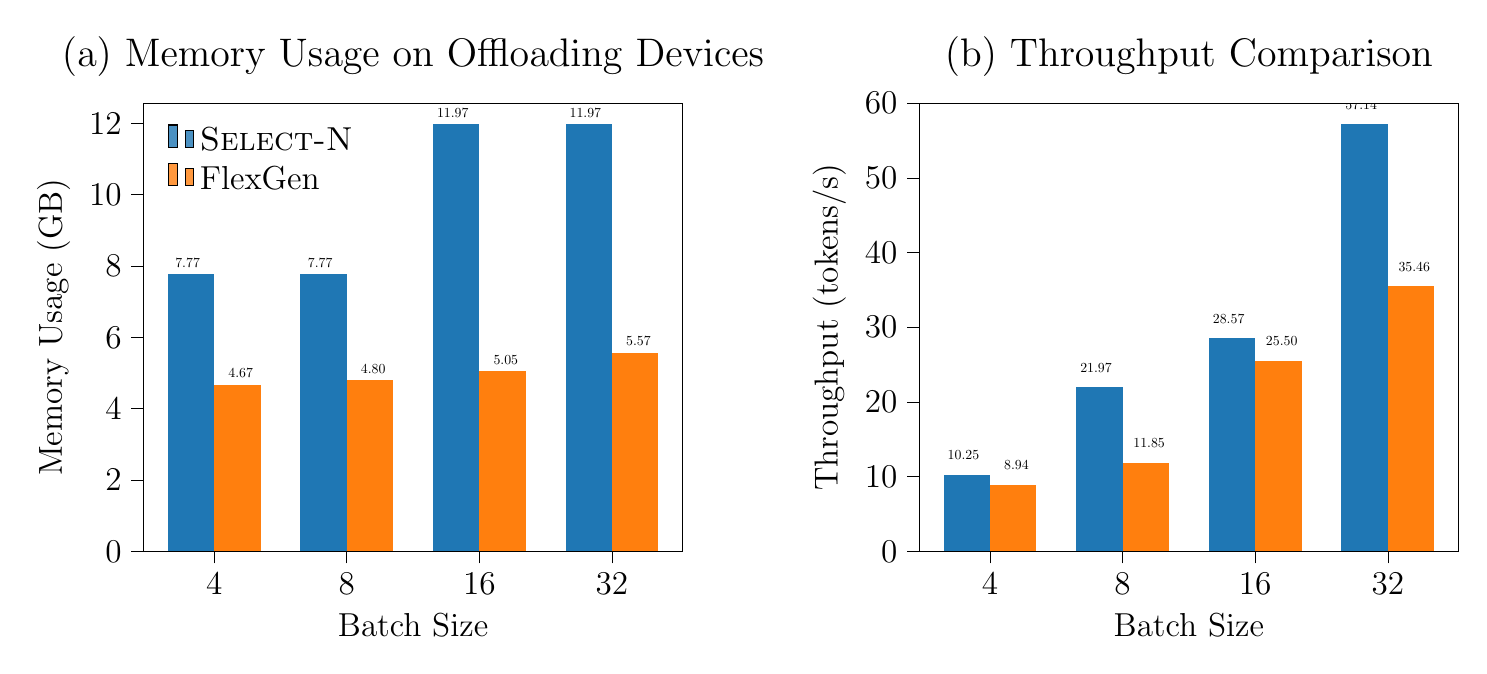
\begin{tikzpicture}

    \definecolor{darkgray176}{RGB}{176,176,176}
    \definecolor{darkorange25512714}{RGB}{255,127,14}
    \definecolor{steelblue31119180}{RGB}{31,119,180}
    
    \begin{groupplot}[group style={group size=2 by 1, horizontal sep=3cm},
      title style={font=\Large},
    label style={font=\large},
    tick label style={font=\large},
    legend style={font=\large}]
    \nextgroupplot[
      legend cell align={left},
      legend style={
        fill opacity=0.8,
        draw opacity=1,
        text opacity=1,
        at={(0.03,0.97)},
        anchor=north west,
        draw=none
      },
      tick align=outside,
      tick pos=left,
      title={(a) Memory Usage on Offloading Devices},
      x grid style={darkgray176},
      xlabel={Batch Size},
      xmin=-0.535, xmax=3.535,
      xtick style={color=black},
      xtick={0,1,2,3},
      xticklabels={4,8,16,32},
      y grid style={darkgray176},
      ylabel={Memory Usage (GB)},
      ymin=0, ymax=12.5685,
      ytick style={color=black}
      ]
      \draw[draw=none,fill=steelblue31119180] (axis cs:-0.35,0) rectangle (axis cs:0,7.77);
      \addlegendimage{ybar,ybar legend,draw=none,fill=steelblue31119180}
      \addlegendentry{\sys}
      
      \draw[draw=none,fill=steelblue31119180] (axis cs:0.65,0) rectangle (axis cs:1,7.77);
      \draw[draw=none,fill=steelblue31119180] (axis cs:1.65,0) rectangle (axis cs:2,11.97);
      \draw[draw=none,fill=steelblue31119180] (axis cs:2.65,0) rectangle (axis cs:3,11.97);
      \draw[draw=none,fill=darkorange25512714] (axis cs:2.77555756156289e-17,0) rectangle (axis cs:0.35,4.672);
      \addlegendimage{ybar,ybar legend,draw=none,fill=darkorange25512714}
      \addlegendentry{FlexGen}
      
      \draw[draw=none,fill=darkorange25512714] (axis cs:1,0) rectangle (axis cs:1.35,4.8);
      \draw[draw=none,fill=darkorange25512714] (axis cs:2,0) rectangle (axis cs:2.35,5.05);
      \draw[draw=none,fill=darkorange25512714] (axis cs:3,0) rectangle (axis cs:3.35,5.57);
      \draw (axis cs:-0.2,7.97) node[
        scale=0.5,
        anchor=base,
        text=black,
        rotate=0.0
      ]{7.77};
      \draw (axis cs:0.8,7.97) node[
        scale=0.5,
        anchor=base,
        text=black,
        rotate=0.0
      ]{7.77};
      \draw (axis cs:1.8,12.17) node[
        scale=0.5,
        anchor=base,
        text=black,
        rotate=0.0
      ]{11.97};
      \draw (axis cs:2.8,12.17) node[
        scale=0.5,
        anchor=base,
        text=black,
        rotate=0.0
      ]{11.97};
      \draw (axis cs:0.2,4.872) node[
        scale=0.5,
        anchor=base,
        text=black,
        rotate=0.0
      ]{4.67};
      \draw (axis cs:1.2,5) node[
        scale=0.5,
        anchor=base,
        text=black,
        rotate=0.0
      ]{4.80};
      \draw (axis cs:2.2,5.25) node[
        scale=0.5,
        anchor=base,
        text=black,
        rotate=0.0
      ]{5.05};
      \draw (axis cs:3.2,5.77) node[
        scale=0.5,
        anchor=base,
        text=black,
        rotate=0.0
      ]{5.57};
      
      \nextgroupplot[
      legend cell align={left},
      legend style={
        fill opacity=0.8,
        draw opacity=1,
        text opacity=1,
        at={(0.03,0.97)},
        anchor=north west,
        draw=none
      },
      tick align=outside,
      tick pos=left,
      title={(b) Throughput Comparison},
      x grid style={darkgray176},
      xlabel={Batch Size},
      xmin=-0.535, xmax=3.535,
      xtick style={color=black},
      xtick={0,1,2,3},
      xticklabels={4,8,16,32},
      y grid style={darkgray176},
      ylabel={Throughput (tokens/s)},
      ymin=0, ymax=59.997,
      ytick style={color=black}
      ]
      \draw[draw=none,fill=steelblue31119180] (axis cs:-0.35,0) rectangle (axis cs:0,10.25);
      \draw[draw=none,fill=steelblue31119180] (axis cs:0.65,0) rectangle (axis cs:1,21.97);
      \draw[draw=none,fill=steelblue31119180] (axis cs:1.65,0) rectangle (axis cs:2,28.57);
      \draw[draw=none,fill=steelblue31119180] (axis cs:2.65,0) rectangle (axis cs:3,57.14);
      \draw[draw=none,fill=darkorange25512714] (axis cs:2.77555756156289e-17,0) rectangle (axis cs:0.35,8.94);
      \draw[draw=none,fill=darkorange25512714] (axis cs:1,0) rectangle (axis cs:1.35,11.85);
      \draw[draw=none,fill=darkorange25512714] (axis cs:2,0) rectangle (axis cs:2.35,25.5);
      \draw[draw=none,fill=darkorange25512714] (axis cs:3,0) rectangle (axis cs:3.35,35.46);
      \draw (axis cs:-0.2,12.25) node[
        scale=0.5,
        anchor=base,
        text=black,
        rotate=0.0
      ]{10.25};
      \draw (axis cs:0.8,23.97) node[
        scale=0.5,
        anchor=base,
        text=black,
        rotate=0.0
      ]{21.97};
      \draw (axis cs:1.8,30.57) node[
        scale=0.5,
        anchor=base,
        text=black,
        rotate=0.0
      ]{28.57};
      \draw (axis cs:2.8,59.14) node[
        scale=0.5,
        anchor=base,
        text=black,
        rotate=0.0
      ]{57.14};
      \draw (axis cs:0.2,10.94) node[
        scale=0.5,
        anchor=base,
        text=black,
        rotate=0.0
      ]{8.94};
      \draw (axis cs:1.2,13.85) node[
        scale=0.5,
        anchor=base,
        text=black,
        rotate=0.0
      ]{11.85};
      \draw (axis cs:2.2,27.5) node[
        scale=0.5,
        anchor=base,
        text=black,
        rotate=0.0
      ]{25.50};
      \draw (axis cs:3.2,37.46) node[
        scale=0.5,
        anchor=base,
        text=black,
        rotate=0.0
      ]{35.46};
      \end{groupplot}
      
      \end{tikzpicture}
       % 插入 TikZ 图
 }
    \caption{(a) Memory usage on the offloading devices for \sys and FlexGen under different batch sizes. 
 (b) Throughput comparison between \sys and FlexGen under different batch sizes.}
    \label{fig:eval2}
\end{figure}


\subsection{Profiling Accuracy}

This subsection evaluates the effectiveness of the \interval analyzer within the \sys framework, 
focusing on verifying whether the \interval value identified during the record-generating phase is indeed optimal. 
To validate this process, we perform experiments using the OPT-6.7B model with a clear separation between the prefill and decoding phases. 
This separation enables the decoding instance to adopt a larger batch size, enhancing throughput in the decoding phase. 
In our experiments, the sequence length is fixed at 64, with a batch size of 16 for the prefill instance and 128 for the decoding instance. 
We set the SLO target at 50\% and use records from the analyzer to determine the optimal \interval value. 
Subsequently, we evaluated the system's performance under non-optimal \interval configurations and recorded the corresponding GPU memory usage for each setting.

The results, shown in Figure~\ref{fig:profileraccu}, highlight the trade-offs inherent in the \interval configuration and the accuracy and necessity of the analyzer in the \sys framework. 
By generating performance records, the optimal \interval values are identified as 3 for the prefill phase and 8 for the decoding phase. 
The optimal \interval values achieve an effective balance by ensuring compliance with both TTFT and TPOT SLOs while minimizing GPU memory usage. 
When \interval is smaller than the optimal value, GPU memory usage is reduced; however, this comes at the cost of SLO violations due to increased latency, 
particularly in the TPOT phase, resulting in degraded throughput. 
In contrast, larger \interval values consistently satisfy the SLO but incur significant memory overhead without measurable performance gains. 
This inefficiency is evident in Figure~\ref{fig:profileraccu}(c), where increasing \interval results in a proportionate consumption of GPU memory while failing to improve latency or throughput.

\begin{figure*}[t]
    \centering
    \resizebox{0.8\textwidth}{!}{
        % This file was created with tikzplotlib v0.10.1.
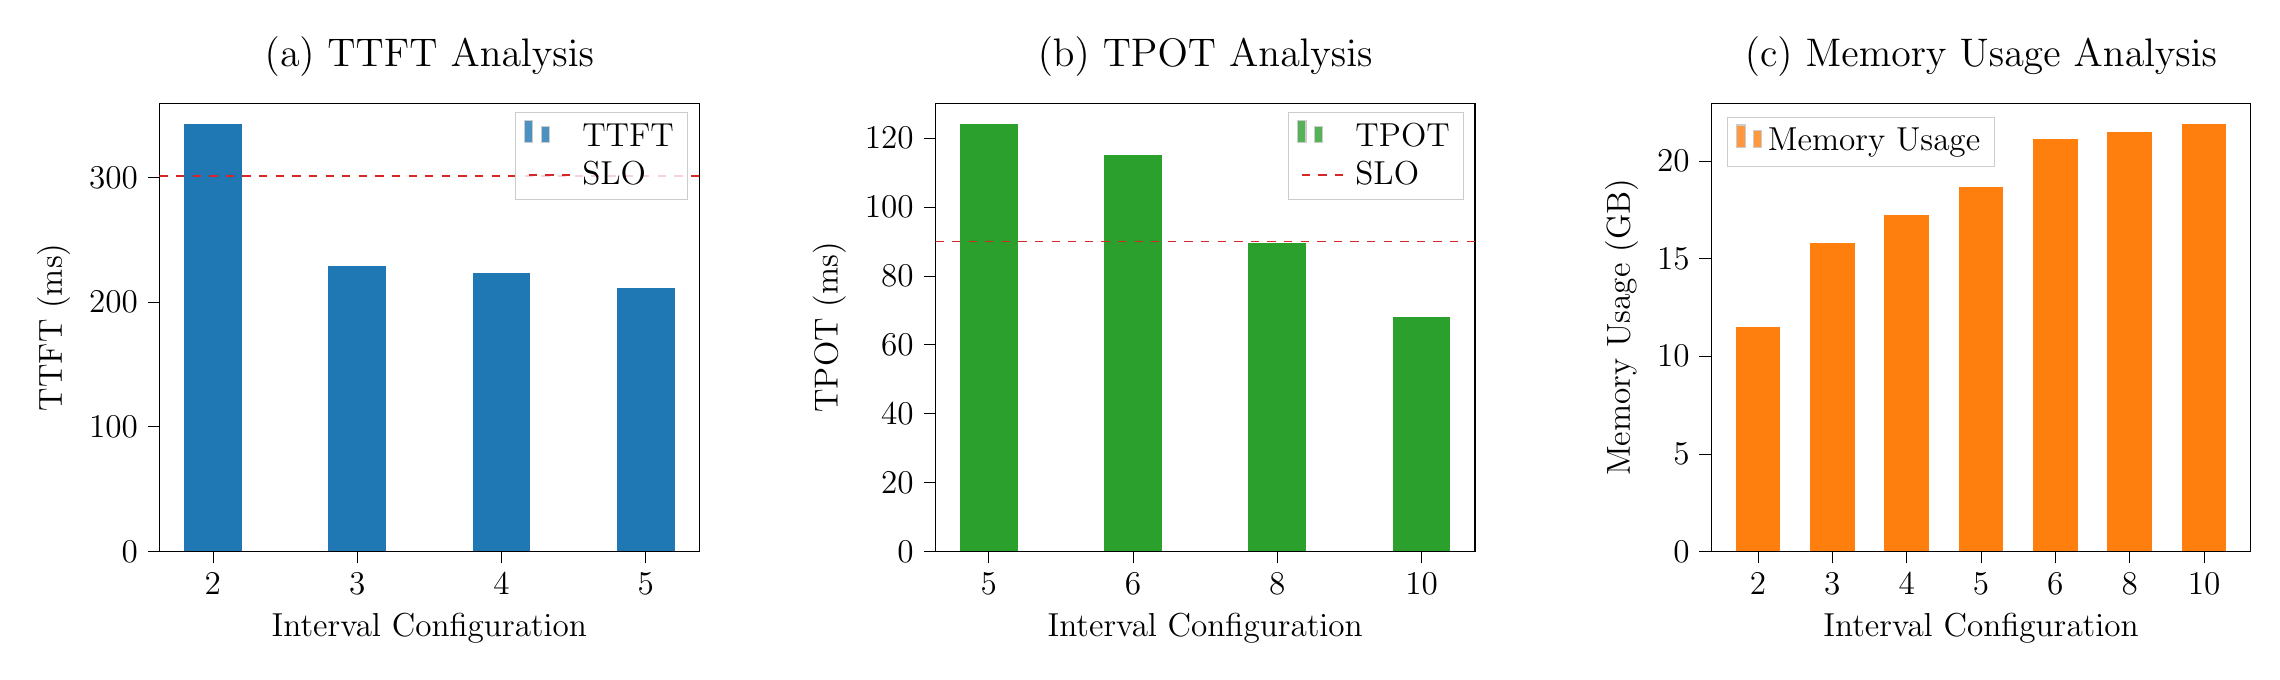
\begin{tikzpicture}

  \definecolor{crimson2143940}{RGB}{214,39,40}
  \definecolor{darkgray176}{RGB}{176,176,176}
  \definecolor{darkorange25512714}{RGB}{255,127,14}
  \definecolor{forestgreen4416044}{RGB}{44,160,44}
  \definecolor{lightgray204}{RGB}{204,204,204}
  \definecolor{steelblue31119180}{RGB}{31,119,180}
  
  \begin{groupplot}[group style={group size=3 by 1, horizontal sep=3cm},
    title style={font=\Large},
    label style={font=\large},
    tick label style={font=\large},
    legend style={font=\large}]
  \nextgroupplot[
  legend cell align={left},
  legend style={fill opacity=0.8, draw opacity=1, text opacity=1, draw=lightgray204},
  tick align=outside,
  tick pos=left,
  title={(a) TTFT Analysis},
  x grid style={darkgray176},
  xlabel={Interval Configuration},
  xmin=-0.37, xmax=3.37,
  xtick style={color=black},
  xtick={0,1,2,3},
  xticklabels={2,3,4,5},
  y grid style={darkgray176},
  ylabel={TTFT (ms)},
  ymin=0, ymax=359.541,
  ytick style={color=black}
  ]
  \draw[draw=none,fill=steelblue31119180] (axis cs:-0.2,0) rectangle (axis cs:0.2,342.42);
  \addlegendimage{ybar,ybar legend,draw=none,fill=steelblue31119180}
  \addlegendentry{TTFT}
  
  \draw[draw=none,fill=steelblue31119180] (axis cs:0.8,0) rectangle (axis cs:1.2,229.157);
  \draw[draw=none,fill=steelblue31119180] (axis cs:1.8,0) rectangle (axis cs:2.2,223.35);
  \draw[draw=none,fill=steelblue31119180] (axis cs:2.8,0) rectangle (axis cs:3.2,210.9);
  \addplot [semithick, crimson2143940, dashed]
  table {%
  -0.37 300.9
  3.37 300.9
  };
  \addlegendentry{SLO}
  
  \nextgroupplot[
  legend cell align={left},
  legend style={fill opacity=0.8, draw opacity=1, text opacity=1, draw=lightgray204},
  tick align=outside,
  tick pos=left,
  title={(b) TPOT Analysis},
  x grid style={darkgray176},
  xlabel={Interval Configuration},
  xmin=-0.37, xmax=3.37,
  xtick style={color=black},
  xtick={0,1,2,3},
  xticklabels={5,6,8,10},
  y grid style={darkgray176},
  ylabel={TPOT (ms)},
  ymin=0, ymax=130.1265,
  ytick style={color=black}
  ]
  \draw[draw=none,fill=forestgreen4416044] (axis cs:-0.2,0) rectangle (axis cs:0.2,123.93);
  \addlegendimage{ybar,ybar legend,draw=none,fill=forestgreen4416044}
  \addlegendentry{TPOT}
  
  \draw[draw=none,fill=forestgreen4416044] (axis cs:0.8,0) rectangle (axis cs:1.2,115.03);
  \draw[draw=none,fill=forestgreen4416044] (axis cs:1.8,0) rectangle (axis cs:2.2,89.388);
  \draw[draw=none,fill=forestgreen4416044] (axis cs:2.8,0) rectangle (axis cs:3.2,68.17);
  \addplot [semithick, crimson2143940, dashed]
  table {%
  -0.369999999999999 90
  3.37 90
  };
  \addlegendentry{SLO}
  
  \nextgroupplot[
  legend cell align={left},
  legend style={
    fill opacity=0.8,
    draw opacity=1,
    text opacity=1,
    at={(0.03,0.97)},
    anchor=north west,
    draw=lightgray204
  },
  tick align=outside,
  tick pos=left,
  title={(c) Memory Usage Analysis},
  x grid style={darkgray176},
  xlabel={Interval Configuration},
  xmin=-0.63, xmax=6.63,
  xtick style={color=black},
  xtick={0,1,2,3,4,5,6},
  xticklabels={2,3,4,5,6,8,10},
  y grid style={darkgray176},
  ylabel={Memory Usage (GB)},
  ymin=0, ymax=22.96875,
  ytick style={color=black}
  ]
  \draw[draw=none,fill=darkorange25512714] (axis cs:-0.3,0) rectangle (axis cs:0.3,11.5);
  \addlegendimage{ybar,ybar legend,draw=none,fill=darkorange25512714}
  \addlegendentry{Memory Usage}
  
  \draw[draw=none,fill=darkorange25512714] (axis cs:0.7,0) rectangle (axis cs:1.3,15.8);
  \draw[draw=none,fill=darkorange25512714] (axis cs:1.7,0) rectangle (axis cs:2.3,17.25);
  \draw[draw=none,fill=darkorange25512714] (axis cs:2.7,0) rectangle (axis cs:3.3,18.69);
  \draw[draw=none,fill=darkorange25512714] (axis cs:3.7,0) rectangle (axis cs:4.3,21.125);
  \draw[draw=none,fill=darkorange25512714] (axis cs:4.7,0) rectangle (axis cs:5.3,21.5);
  \draw[draw=none,fill=darkorange25512714] (axis cs:5.7,0) rectangle (axis cs:6.3,21.875);
  \end{groupplot}
  
  \end{tikzpicture}
   % 插入 TikZ 图
 }
    \caption{The TTFT, TPOT, and memory usage of \sys under different \interval configurations. 
 The red dashed lines represent the SLO. The optimal \interval is 3 in (a) and 8 in (b).}
    \label{fig:profileraccu}
\end{figure*}


\subsection{Bandwidth contention}

We conduct experiments simulating a scenario where two GPUs share PCIe bandwidth. 
In this setup, one GPU runs the OPT-13B model while the other GPU runs the LLaMA-13B model simultaneously. 
Since both models are too large to fully fit into GPU memory, offloading strategies were required to enable the models to run successfully.
That creates a high-bandwidth contention environment as both GPUs perform offloading and data transfers concurrently. 
The sequence length was set to 64, and batch sizes of 8, 16, and 32 were tested for both tasks.

To address the contention, \sys dynamically adjusts the \interval values for both tasks, ensuring that neither exceeded the predefined SLO. 
Since it is not feasible to test the computation time in a naive mode where the entire model fits into GPU memory, we could not define the SLO as a percentage of naive execution time. 
Instead, we set the SLO as a fixed TPOT threshold of 100ms. 
This value is significantly higher than typical human reading speeds and provides a stringent and practical target for evaluating performance under high-bandwidth contention. 
We also compare the performance of \sys with FlexGen on the GPU running the OPT-13B task with the same batch sizes. 
This comparison highlights \sys's ability to adaptively manage contention on the shared PCIe bandwidth, compared to FlexGen's static offloading strategy.

The results, shown in Figure~\ref{fig:evalband}, illustrate the TPOT performance of \sys and FlexGen under varying batch sizes in a bandwidth contention scenario. 
FlexGen exhibits acceptable performance at the largest batch size tested (32) but violates the SLO at smaller batch sizes (8 and 16) due to its inability to adapt to varying PCIe transfer demands. 
In contrast, \sys consistently maintains TPOT below the SLO across all batch sizes by dynamically adjusting the \interval values of the two tasks, 
effectively mitigating bandwidth contention and ensuring balanced resource utilization. 
This adaptability enables \sys to achieve 2.9\X higher throughput compared to FlexGen at smaller batch sizes on the OPT-13B task.


\begin{figure}[t]
    \centering
    \resizebox{0.6\columnwidth}{!}{
        % This file was created with tikzplotlib v0.10.1.
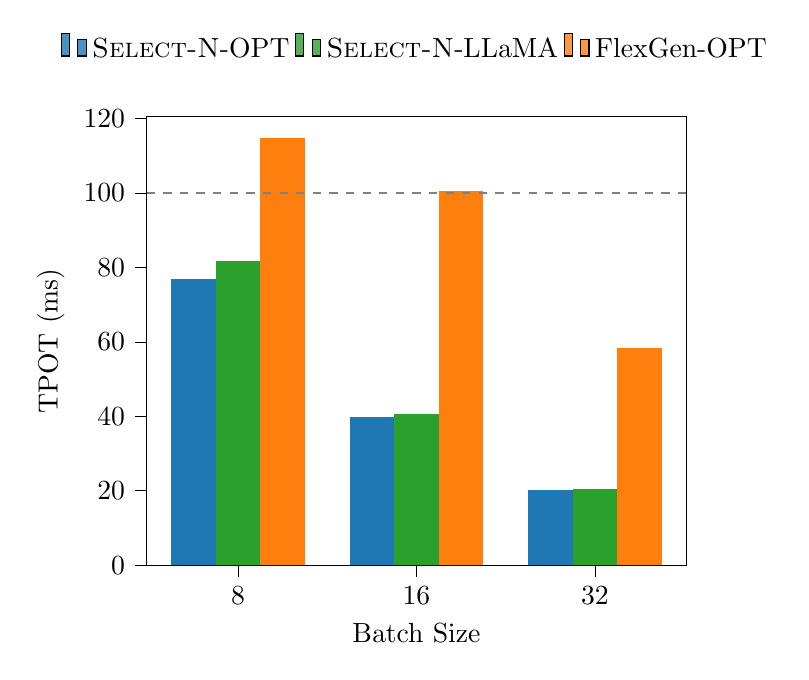
\begin{tikzpicture}

  \definecolor{darkgray176}{RGB}{176,176,176}
  \definecolor{darkorange25512714}{RGB}{255,127,14}
  \definecolor{forestgreen4416044}{RGB}{44,160,44}
  \definecolor{gray}{RGB}{128,128,128}
  \definecolor{steelblue31119180}{RGB}{31,119,180}
  
  \begin{axis}[
  legend cell align={left},
  legend columns=3,
  legend style={fill opacity=0.8, draw opacity=1, text opacity=1, at={(0.5,1.2)}, anchor=north, draw=none},
  tick align=outside,
  tick pos=left,
  x grid style={darkgray176},
  xlabel={Batch Size},
  xmin=-0.5125, xmax=2.5125,
  xtick style={color=black},
  xtick={0,1,2},
  xticklabels={8,16,32},
  y grid style={darkgray176},
  ylabel={TPOT (ms)},
  ymin=0, ymax=120.4875,
  ytick style={color=black}
  ]
  \draw[draw=none,fill=steelblue31119180] (axis cs:-0.375,0) rectangle (axis cs:-0.125,76.99);
  \addlegendimage{ybar,ybar legend,draw=none,fill=steelblue31119180}
  \addlegendentry{\sys-OPT}
  
  \draw[draw=none,fill=steelblue31119180] (axis cs:0.625,0) rectangle (axis cs:0.875,39.91);
  \draw[draw=none,fill=steelblue31119180] (axis cs:1.625,0) rectangle (axis cs:1.875,20.16);
  \draw[draw=none,fill=forestgreen4416044] (axis cs:-0.125,0) rectangle (axis cs:0.125,81.756375);
  \addlegendimage{ybar,ybar legend,draw=none,fill=forestgreen4416044}
  \addlegendentry{\sys-LLaMA}
  
  \draw[draw=none,fill=forestgreen4416044] (axis cs:0.875,0) rectangle (axis cs:1.125,40.6360625);
  \draw[draw=none,fill=forestgreen4416044] (axis cs:1.875,0) rectangle (axis cs:2.125,20.31803125);
  \draw[draw=none,fill=darkorange25512714] (axis cs:0.125,0) rectangle (axis cs:0.375,114.75);
  \addlegendimage{ybar,ybar legend,draw=none,fill=darkorange25512714}
  \addlegendentry{FlexGen-OPT}
  
  \draw[draw=none,fill=darkorange25512714] (axis cs:1.125,0) rectangle (axis cs:1.375,100.43);
  \draw[draw=none,fill=darkorange25512714] (axis cs:2.125,0) rectangle (axis cs:2.375,58.44);
  \addplot [gray, dashed, forget plot]
  table {%
  -0.5125 100
  2.5125 100
  };
  \end{axis}
  
  \end{tikzpicture}
   % 插入 TikZ 图
 }
    \caption{TPOT comparison of \sys (OPT-13B and LLaMA-13B models) and FlexGen (OPT-13B model) under contention environments across different batch sizes.
 The dashed line represents the SLO.}
    \label{fig:evalband}
\end{figure}



\subsection{Benefits of \sys}
\label{sec:benefits}

\PN{Supporting larger models.}
\sys is capable of supporting models whose memory demands exceed the GPU memory capacity, as demonstrated in experiments with the LLaMA-13B and OPT-13B models. 
Figure~\ref{fig:eval3} presents the TPOT performance of LLaMA-13B and OPT-13B, respectively, under varying batch sizes. Both models, 
which require memory beyond the 24GB GPU capacity in our setup, were successfully executed using \sys. 
TPOT values below 100 ms are higher than the normal human reading speed, indicating that such latencies allow for efficient and real-time text generation. 
In our experiments, the TPOT values for both LLaMA-13B and OPT-13B remained consistently below 100ms across all tested batch sizes, 
confirming that \sys not only enables the execution of these large-scale models but also ensures efficient performance suitable for real-world applications.

\begin{figure}[t]
    \centering
    \resizebox{\columnwidth}{!}{
        % This file was created with tikzplotlib v0.10.1.
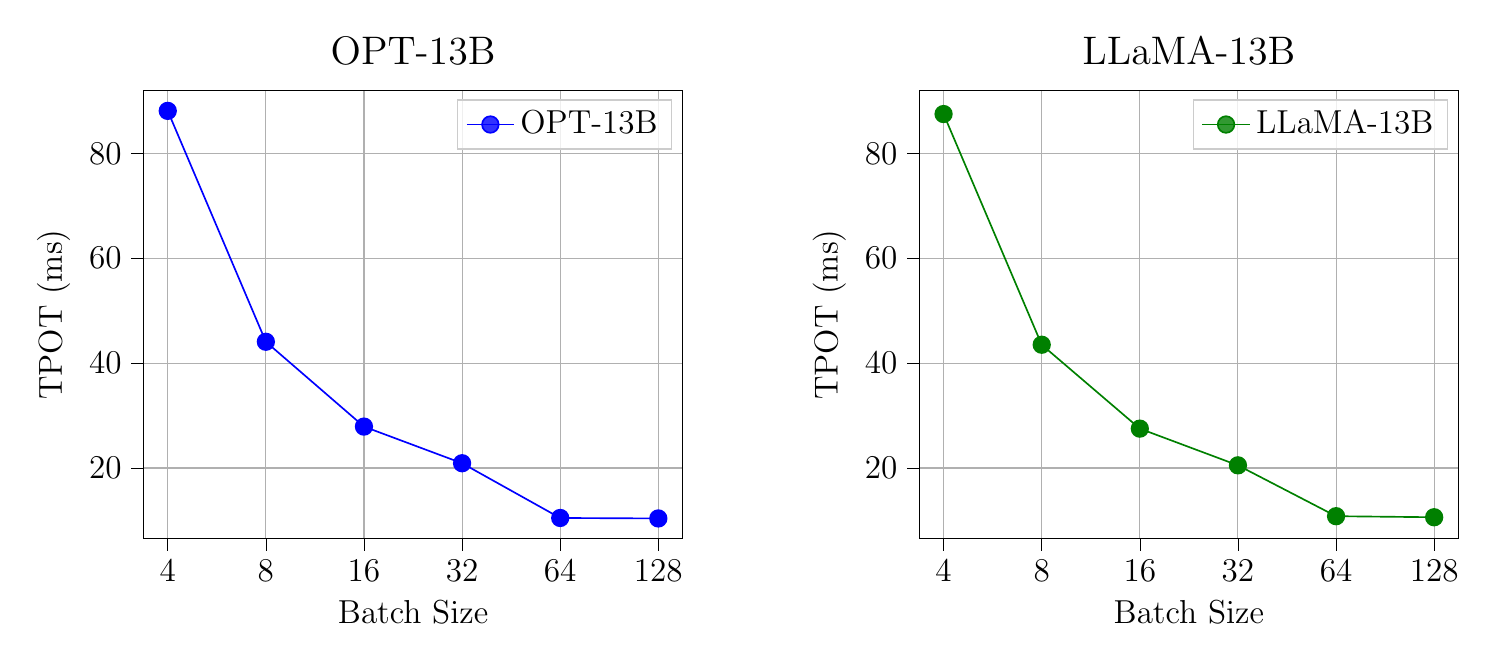
\begin{tikzpicture}

    \definecolor{darkgray176}{RGB}{176,176,176}
    \definecolor{green}{RGB}{0,128,0}
    \definecolor{lightgray204}{RGB}{204,204,204}
    
    \begin{groupplot}[group style={group size=2 by 1, horizontal sep=3cm},
        title style={font=\Large},
    label style={font=\large},
    tick label style={font=\large},
    legend style={font=\large}]
    \nextgroupplot[
    legend cell align={left},
    legend style={fill opacity=0.8, draw opacity=1, text opacity=1, draw=lightgray204},
    tick align=outside,
    tick pos=left,
    title={OPT-13B},
    x grid style={darkgray176},
    xlabel={Batch Size},
    xmajorgrids,
    xmin=-0.25, xmax=5.25,
    xtick style={color=black},
    xtick={0,1,2,3,4,5},
    xtick={0,1,2,3,4,5},
    xticklabels={4,8,16,32,64,128},
    xticklabels={4,8,16,32,64,128},
    y grid style={darkgray176},
    ylabel={TPOT (ms)},
    ymajorgrids,
    ymin=6.4835, ymax=91.9865,
    ytick style={color=black}
    ]
    \addplot [semithick, blue, mark=*, mark size=3, mark options={solid}]
    table {%
    0 88.1
    1 44.066
    2 27.8875
    3 20.9
    4 10.46
    5 10.37
    };
    \addlegendentry{OPT-13B}
    
    \nextgroupplot[
    legend cell align={left},
    legend style={fill opacity=0.8, draw opacity=1, text opacity=1, draw=lightgray204},
    scaled y ticks=manual:{}{\pgfmathparse{#1}},
    tick align=outside,
    tick pos=left,
    title={LLaMA-13B},
    x grid style={darkgray176},
    xlabel={Batch Size},
    xmajorgrids,
    xmin=-0.25, xmax=5.25,
    xtick style={color=black},
    xtick={0,1,2,3,4,5},
    xtick={0,1,2,3,4,5},
    xticklabels={4,8,16,32,64,128},
    xticklabels={4,8,16,32,64,128},
    y grid style={darkgray176},
    ylabel={TPOT (ms)},
    ymajorgrids,
    ymin=6.4835, ymax=91.9865,
    ytick style={color=black},
    % yticklabels={}
    ]
    \addplot [semithick, green, mark=*, mark size=3, mark options={solid}]
    table {%
    0 87.5
    1 43.5
    2 27.5
    3 20.5
    4 10.8
    5 10.6
    };
    \addlegendentry{LLaMA-13B}
    \end{groupplot}
    
    \end{tikzpicture}
     % 插入 TikZ 图
 }
    \caption{TPOT of OPT-13B and LLaMA-13B models using \sys.}
    \label{fig:eval3}
\end{figure}

\PN{Supporting more input and output tokens.}
To evaluate the capability of \sys in generating longer output sequences and supporting larger batch sizes and/or sequence lengths, we leverage a critical metric:
the maximum allocatable length (\textit{max length}). 
This metric is computed as 
\[
\textit{max length} = \textit{batch size} \times (\textit{sequence length} + \textit{output length}),
\]
where the term captures the total number of tokens that the system can handle for a single model instance. 
The \textit{max length} is directly determined by the number of GPU blocks allocatable via the vLLM backend, which dynamically manages GPU memory to optimize allocation. 
A higher \textit{max length} indicates the system’s ability to support larger batch sizes, longer input sequences, and extended output sequences.

In our experiments, we use the Qwen2-beta-7B model, which supports a maximum position embedding size of 32,768 tokens. 
This choice is deliberate, as Qwen2-beta-7B significantly exceeds the position embedding limits of other models like OPT and LLaMA, 
ensuring that the system remains capable of processing long input sequences without being constrained by the model's internal architecture. 

The results in Figure~\ref{fig:eval4} show that, by adjusting the offloading intervals, \sys achieves varying degrees of memory savings for model inference. 
When the interval value is smaller, a larger proportion of the model's parameters is offloaded to CPU memory, significantly reducing the GPU memory footprint. 
This allows \sys to allocate more GPU memory for token processing, thereby increasing the maximum allocatable length. 
As a result, the system can support larger batch sizes, longer input sequences, or extended output sequences under smaller interval settings, which helps to improve throughput.


\begin{figure}[t]
    \centering
    \resizebox{0.5\columnwidth}{!}{
        % This file was created with tikzplotlib v0.10.1.
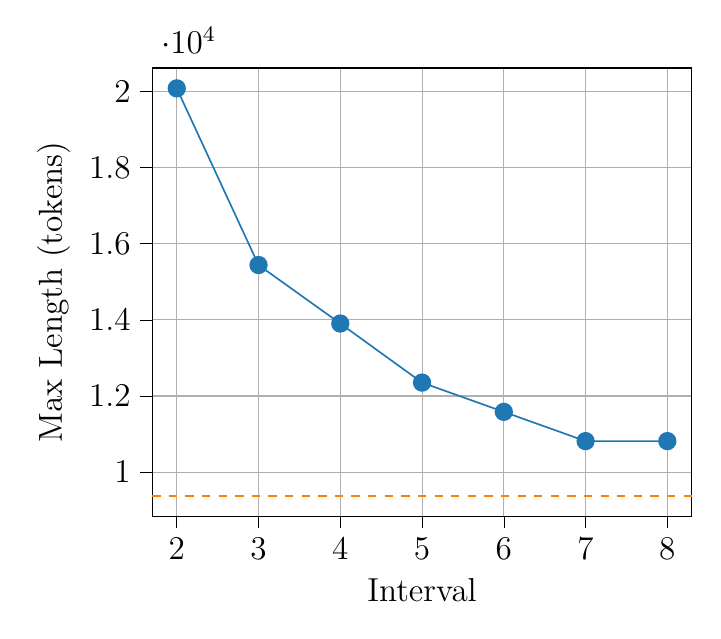
\begin{tikzpicture}

    \definecolor{darkgray176}{RGB}{176,176,176}
    \definecolor{darkorange25512714}{RGB}{255,127,14}
    \definecolor{steelblue31119180}{RGB}{31,119,180}
    
    \begin{axis}[
        title style={font=\Large},
        label style={font=\large},
        tick label style={font=\large},
        legend style={font=\large},
    tick align=outside,
    tick pos=left,
    x grid style={darkgray176},
    xlabel={Interval},
    xmajorgrids,
    xmin=1.7, xmax=8.3,
    xtick style={color=black},
    y grid style={darkgray176},
    ylabel={Max Length (tokens)},
    ymajorgrids,
    ymin=8840.8, ymax=20615.2,
    ytick style={color=black}
    ]
    \addplot [semithick, steelblue31119180, mark=*, mark size=3, mark options={solid}]
    table {%
    2 20080
    3 15440
    4 13904
    5 12352
    6 11584
    7 10816
    8 10816
    };
    \addplot [semithick, darkorange25512714, dashed]
    table {%
    1.7 9376
    8.3 9376
    };
    \end{axis}
    
    \end{tikzpicture}
     % 插入 TikZ 图
 }
    \caption{Maximum prompt length the model can process under different \interval settings.
 The dashed line represents the maximum length in the naive mode.}
    \label{fig:eval4}
\end{figure}


%-------------------------------------------------------------------------------
\section{Related Work}
%-------------------------------------------------------------------------------
\label{sec:relwk}

\PN{Efficient LLM serving.} 
Several recent studies address these challenges by proposing methods to enhance system performance and resource efficiency in LLM inference. 
Orca\cite{orca} introduces continuous batching to enhance GPU throughput. 
vLLM\cite{vllm} leverages PageAttention to optimize KV cache memory usage, enabling efficient resource allocation. 
SARATHI\cite{SARATHI} adopts a chunked-prefill strategy, dividing prefill requests into smaller chunks while combining them with decoding requests to achieve better hardware utilization. 
StreamingLLM\cite{StreamingLLM} extends LLM capabilities by allowing the generation of sequence lengths beyond their original training limits. 
\sys builds on some of these techniques like vLLM, and is designed to work in parallel with other approaches to further enhance performance and resource efficiency.

\PN{Offloading techniques.}
Existing works have explored various techniques to improve large-scale model inference performance, particularly on resource-constrained hardware. 
Systems such as DeepSpeed ZeRO-Inference\cite{zero-infer} and Hugging Face Accelerate\cite{huggingface} adopt offloading strategies originally designed for training scenarios. 
Infinite-LLM\cite{lin2024infinitellmefficientllmservice} manages the utilization of all GPU and CPU memory resources to store the KV cache.
These approaches may still cause computation to stall as they do not ensure data readiness at the required time.
InfiniGen\cite{infinigen} mitigates KV cache fetch overhead by speculatively prefetching essential KV entries, improving cache management efficiency. 
Neo\cite{jiangxuanlin} offloads part of attention compute and KV cache states from GPU to CPU to balance compute and memory resources.
These two works cannot handle models that exceed the GPU memory capacity, making them orthogonal to our approach.

\PN{Scheduling systems.} 
Recent works have explored efficient resource scheduling and allocation strategies for deep learning tasks, focusing on optimizing throughput\cite{pollux}, 
heterogeneous-aware scheduling\cite{sia}, preemption and latency-aware scheduling\cite{Clockwork, SHEPHERD}, 
and improving resource utilization through model parallelism\cite{AlpaServe} or iteration-level preemptive scheduling to mitigate queueing delays\cite{fastserve}.
There are also concurrent works that employ disaggregation techniques to decouple and balance resource allocation, 
improving efficiency in LLM inference, such as Splitwise\cite{splitwise}, TetriInfer\cite{TetriInfer}, DéjàVu\cite{dejavu}, and Distserve\cite{distserve}
\sys is orthogonal to the large body of work on scheduling, as its separation of prefill and decoding stages can be implemented using any of the aforementioned approaches.



\section{Conclusion}

This paper is one of the first attempts to understand, categorize, and detect \termname terms and conditions on shopping websites. These terms, which can significantly impact consumer trust and satisfaction, have not been extensively studied. By highlighting the prevalence and types of \termname terms, we hope to pave the way for increased awareness and further research in this area. We develop an automated data collection and topic modeling pipeline, analyzing \termcnt terms from \websitecnt websites to create a taxonomy for \termname terms. This taxonomy includes \termtypecnt types across \termcatcnt categories, covering purchase and billing, post-purchase activities, account termination, and legal aspects.


\platform is the first study to evaluate the effectiveness of LLMs in identifying \termname terms. Using a fine-tuned GPT-4o model on a manually annotated dataset, \platform achieves an F1 score of 94.6\% with a false positive rate of 2.3\%. In large-scale deployment, we find that approximately \websitepct of shopping websites in the Tranco top 100,000 contain at least one category of \termname terms. Our qualitative analysis shows that current ecosystem defenses are inadequate to protect users from these terms, that less popular websites are more likely to include \termname terms, and that there is a correlation between \termname terms and user dissatisfaction.





% Ack: thank openai and renuka
\section*{Acknowledgments}

The authors would like to thank Renuka Kumar for her valuable input and suggestions during the early stages of this project.  This work is supported by a gift from the OpenAI Cybersecurity Grant program. Any opinions, findings, conclusions, or recommendations expressed in this material are those of the authors
and do not necessarily reflect the views of OpenAI.


% \section*{Acknowledgements}
This is acknowledgment.


% % use with balance package
%%%%%%%%%%%%%%%%%%%%%%%%%%%%%%%%%%%%%%%%%%%%%%%%%%%%%%
% \balance
%%%%%%%%%%%%%%%%%%%%%%%%%%%%%%%%%%%%%%%%%%%%%%%%%%%%%%

% use multicol if you are using pygmentize package along with multicol package
%%%%%%%%%%%%%%%%%%%%%%%%%%%%%%%%%%%%%%%%%%%%%%%%%%%%%%
\onecolumn
\begin{multicols}{2}
%%%%%%%%%%%%%%%%%%%%%%%%%%%%%%%%%%%%%%%%%%%%%%%%%%%%%%

\nocite{*}

\bibliographystyle{abbrvnat}
\footnotesize
\setlength{\bibsep}{3pt}
\bibliography{p}

% for multicol
%%%%%%%%%%%%%%%%%%%%%%%%%%%%%%%%%%%%%%%%%%%%%%%%%%%%%%
\end{multicols}
%%%%%%%%%%%%%%%%%%%%%%%%%%%%%%%%%%%%%%%%%%%%%%%%%%%%%%

\end{document}

